\newcommand{\institut}{Institut f\"ur Telekommunikationssysteme}
\newcommand{\fachgebiet}{Nachrichten\"ubertragung}
\newcommand{\veranstaltung}{Praktikum Nachrichten\"ubertragung}
\newcommand{\pdfautor}{Dirk Babendererde (321 836), Thomas Kapa (325 219)}
\newcommand{\autor}{Dirk Babendererde (321 836)\\ Thomas Kapa (325 219)}
\newcommand{\gruppe}{Gruppe:}
\newcommand{\betreuer}{Betreuer: Lieven Lange}


\newcommand{\pdftitle}{Nachrichtenuebertragung\ Praktikum\ 05}
\newcommand{\prototitle}{Praktikum 05 \\ Pulsamplitudenmodulation und nichtideale Abtastung}

\input{../../packages/tu_header_9}

% damit das outline funktioniert noch mal:
\begin{document}


%     \lstinputlisting{./praktikum6.sce}

%---------------------------------------------------------------------
%---------------------------------------------------------------------
%---------------------------------------------------------------------

\section{Vorbereitung}
\begin{quote}
    
    
    \begin{figure}[H]
        \centering
        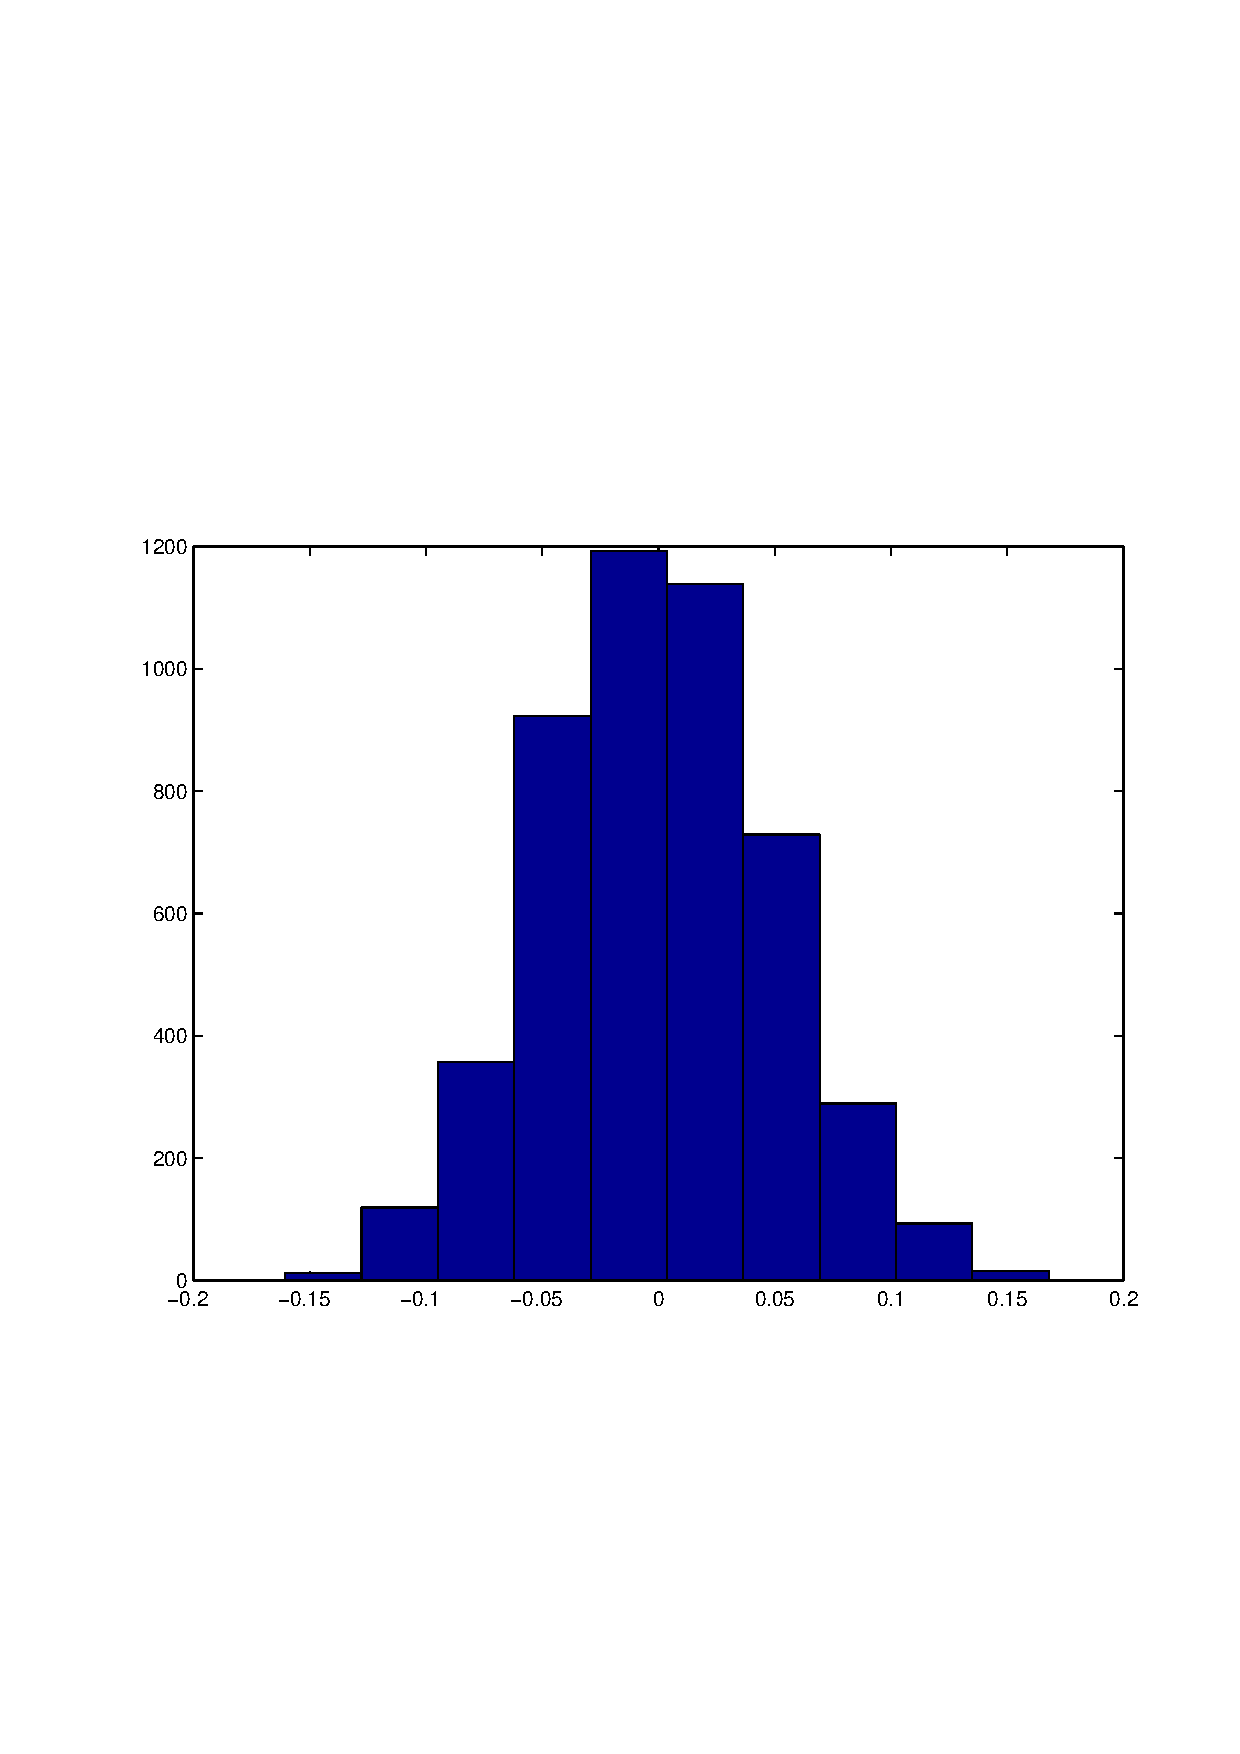
\includegraphics[scale=0.7, trim = 2cm 7cm 1cm 8cm, clip]{Bilder/PCM_Test}
        \caption{Testkennlinie des PCM-Analyse Scriptes}
        \label{fig:PCM_Test}
    \end{figure}
    
    \vspace{2em}
    
    In Abbildung \ref{fig:PCM_Test} ist die PCM-Encoder-Kennlinie einer Messreihe zu sehen, die mit einem nicht
    linearen Quantisierer quantisiert wurde. Dabei werden die Werte um 0 herum wesentlich genauer und die
    Werte im größeren Spannungsbreich seltener abgetastet. Dies kann von Vorteil sein, wenn die Werte um 0 häufiger
    auftreten und somit für die Messung interessanter sind.\\
    
    
    
    
    \TODO{Blockschaltbild? erklärung?}
    
    
    
    
\end{quote}


\section{Labordurchführung}
\begin{quote}
    
    
    \subsection{Encoderkennlinie}
    \begin{quote}
        
        Es soll die PCM-Encoder-Kennlinie aufgenommen werden.
        Dazu wird das PCM-Encoder-Modul des ETT101 genutzt. Zunächst wird als Clocksignal an den Eingang CLK das
        100 kHz DIGITAL Signal des Master Signals-Modul gelegt. Anschließend wird als Eingang in INPUT 1 ein
        symmetrisches Dreiecksignal mit einer Amplitude von 2,5 Volt angelegt (2,5 Volt, damit für über 2 und unter -2 Volt
        die Codewörter 1111 1111 und 0000 0000 ausgegeben werden) und der Schalter auf PCM gestellt.
        Die beiden Ausgänge FS (Rahmensignal) und PCM (Pulsecode) werden auf die beiden Eingänge des Addierers gegeben. Da
        beide Signale 5 Volt high und 0 Volt low ausgeben, wird die Verstärkung für das PCM-Signal auf 0 gestellt und die
        Verstärkung für das Rahmensignal auf 8/5 gestellt, um die Anforderungen aus der Aufgabenstellung zu erfüllen.
        Mit dem Picoscope werden die Summe aus Rahmensignal und Pulscodesignal und eine steigende Flanke des Zeitignals
        gemessen und angezeigt.
        
        
    \end{quote}
    
    \subsection{Quantisierungsfehler, Kodieren, Dekodieren}
    
    \begin{quote}
        
        Um den Quantisierungsfehler bestimmen zu können, werden das Eingangssignal und das dekodierte Signal benötigt. Zur
        Dekodierung wird das PCM Decoder-Modul genutzt. Die Eingänge FS, PCM DATA un CLK werden mit ihren jeweiligen
        Gegenstücken des PCM Encoder-Moduls verbunden. Anschließend wird das Signal am OUTPUT 1 zusammen mit dem
        Eingangsignal dem Picoscope zugeführt.\\
        
        
        
        
        
    \end{quote}
    
    
    
    
\end{quote}

\section{Auswertung \& Theorie}
\begin{quote}
    
    \subsection{Encoderkennlinie}
    
    \begin{quote}
        
    \begin{figure}[H]
        \centering
        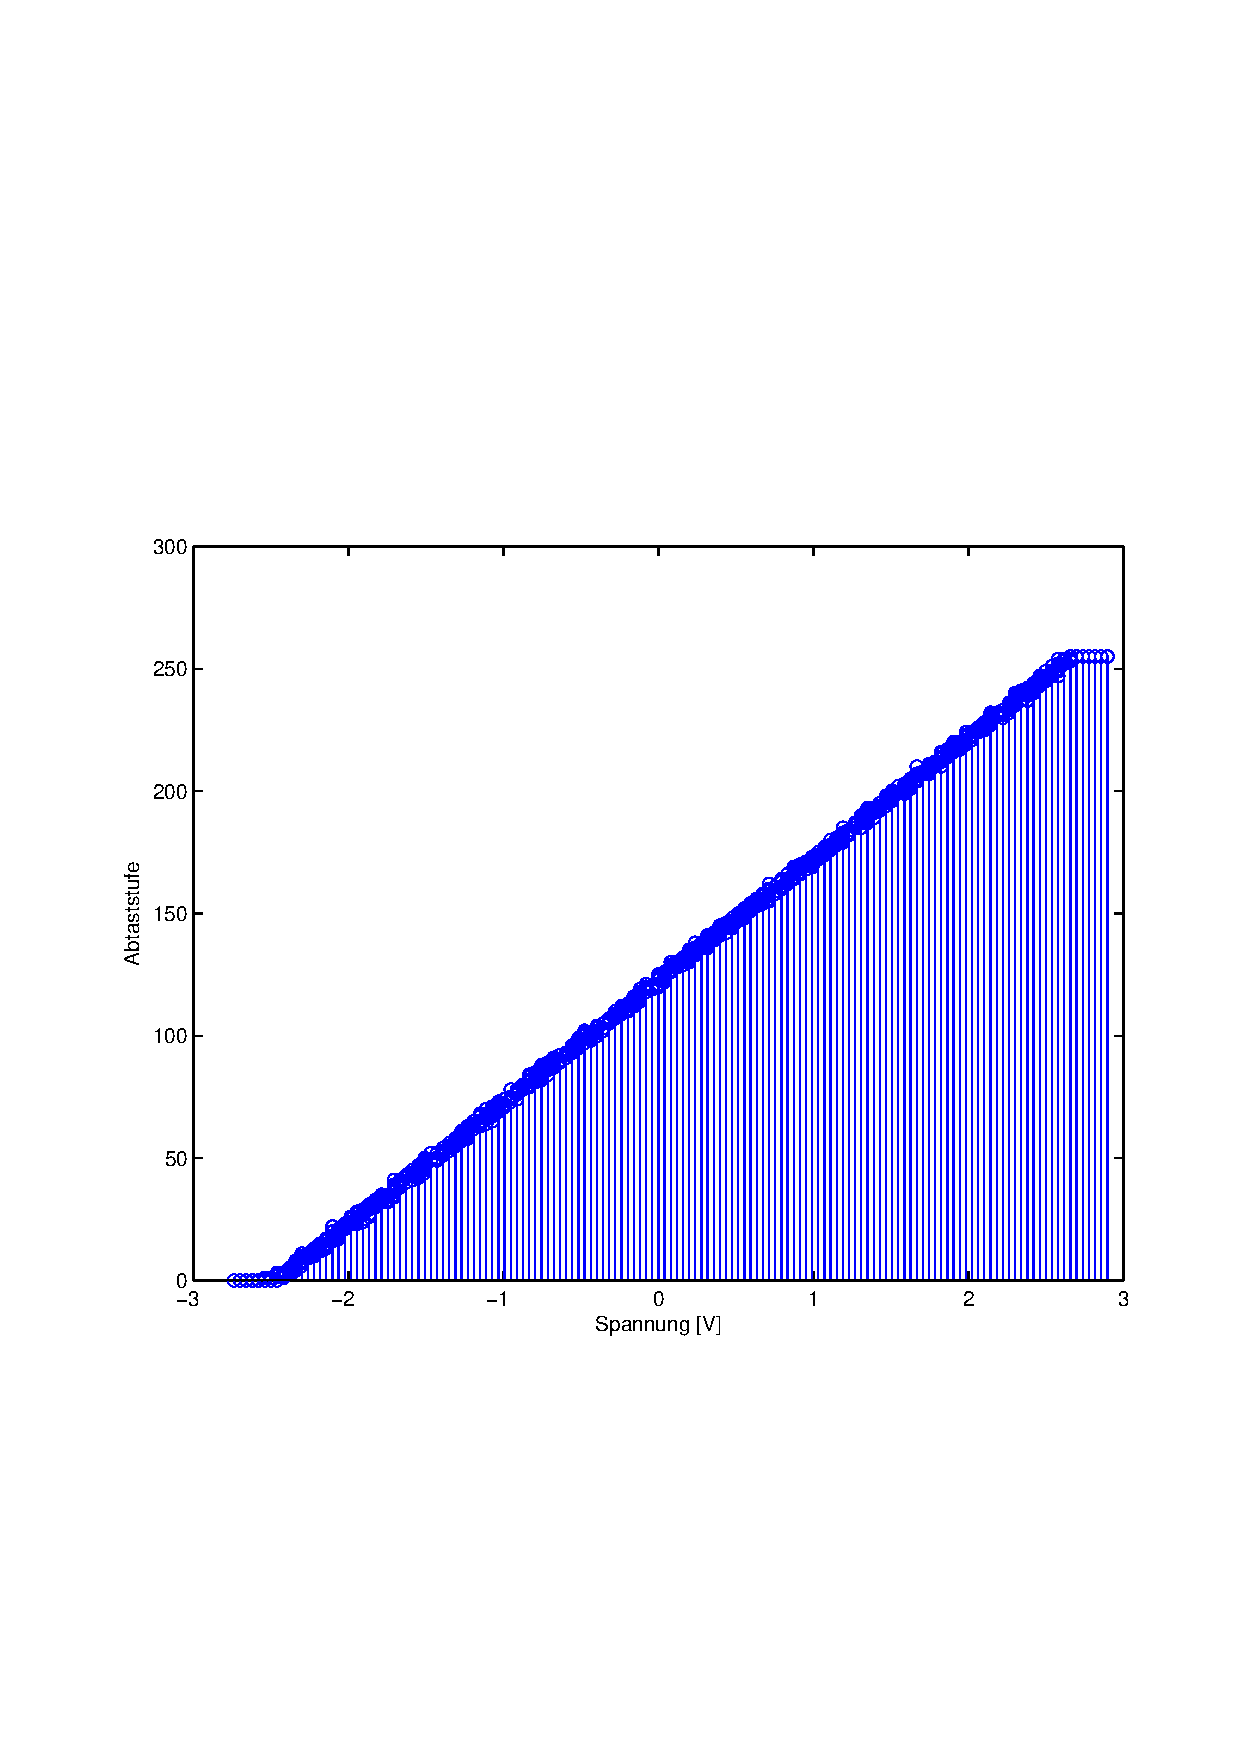
\includegraphics[scale=0.7, trim = 2cm 7cm 1cm 8cm, clip]{Bilder/PCM_Test_auswertung}
        \caption{PCM-Encoderkennlinie der steigenden Dreiecksflanke}
        \label{fig:PCM_Test_dreieck}
    \end{figure}
    
    In Abbildung \ref{fig:PCM_Test_dreieck} erkennt man im Gegensatz zu der Abbildung \ref{fig:PCM_Test} in der
    Vorbereitungsaufgabe eine lineare Encoder-Kennlinie. Die im Labor mit dem PCM-Modul aufgenommenen Messwerte wurden
    also mit einem linearen Quantisierer aufgenommen.
    
    \end{quote}
    
    
    \subsection{Quantisierungfehler}
    
    \begin{quote}
        Das Signal besitzt in dieser Form noch einen Mittelwert (Offset), welcher mit der Funktion mean in Matlab ermittelt
        werden kann und vom Signal abgezogen wird. Da weiterhin das Signal durch den Kodier- und Dekodiervorgang eine
        Dämpfung und einen Delay erfährt, wird das dekodierte Signal mit Hilfe von Matlab verstärkt und mit der Kreuzkorrelation
        um die erfahrene Verzögerung verschoben. Das Ergebnis ist in Abb. \ref{fig:100kHz_sin_rek_angepasst} zu sehen. \\
        
        \begin{center}
            \begin{tabular}{ll}
            
            \hspace{-4cm}
                \begin{minipage}{0.6\textwidth}
                    \begin{figure}[H]
                        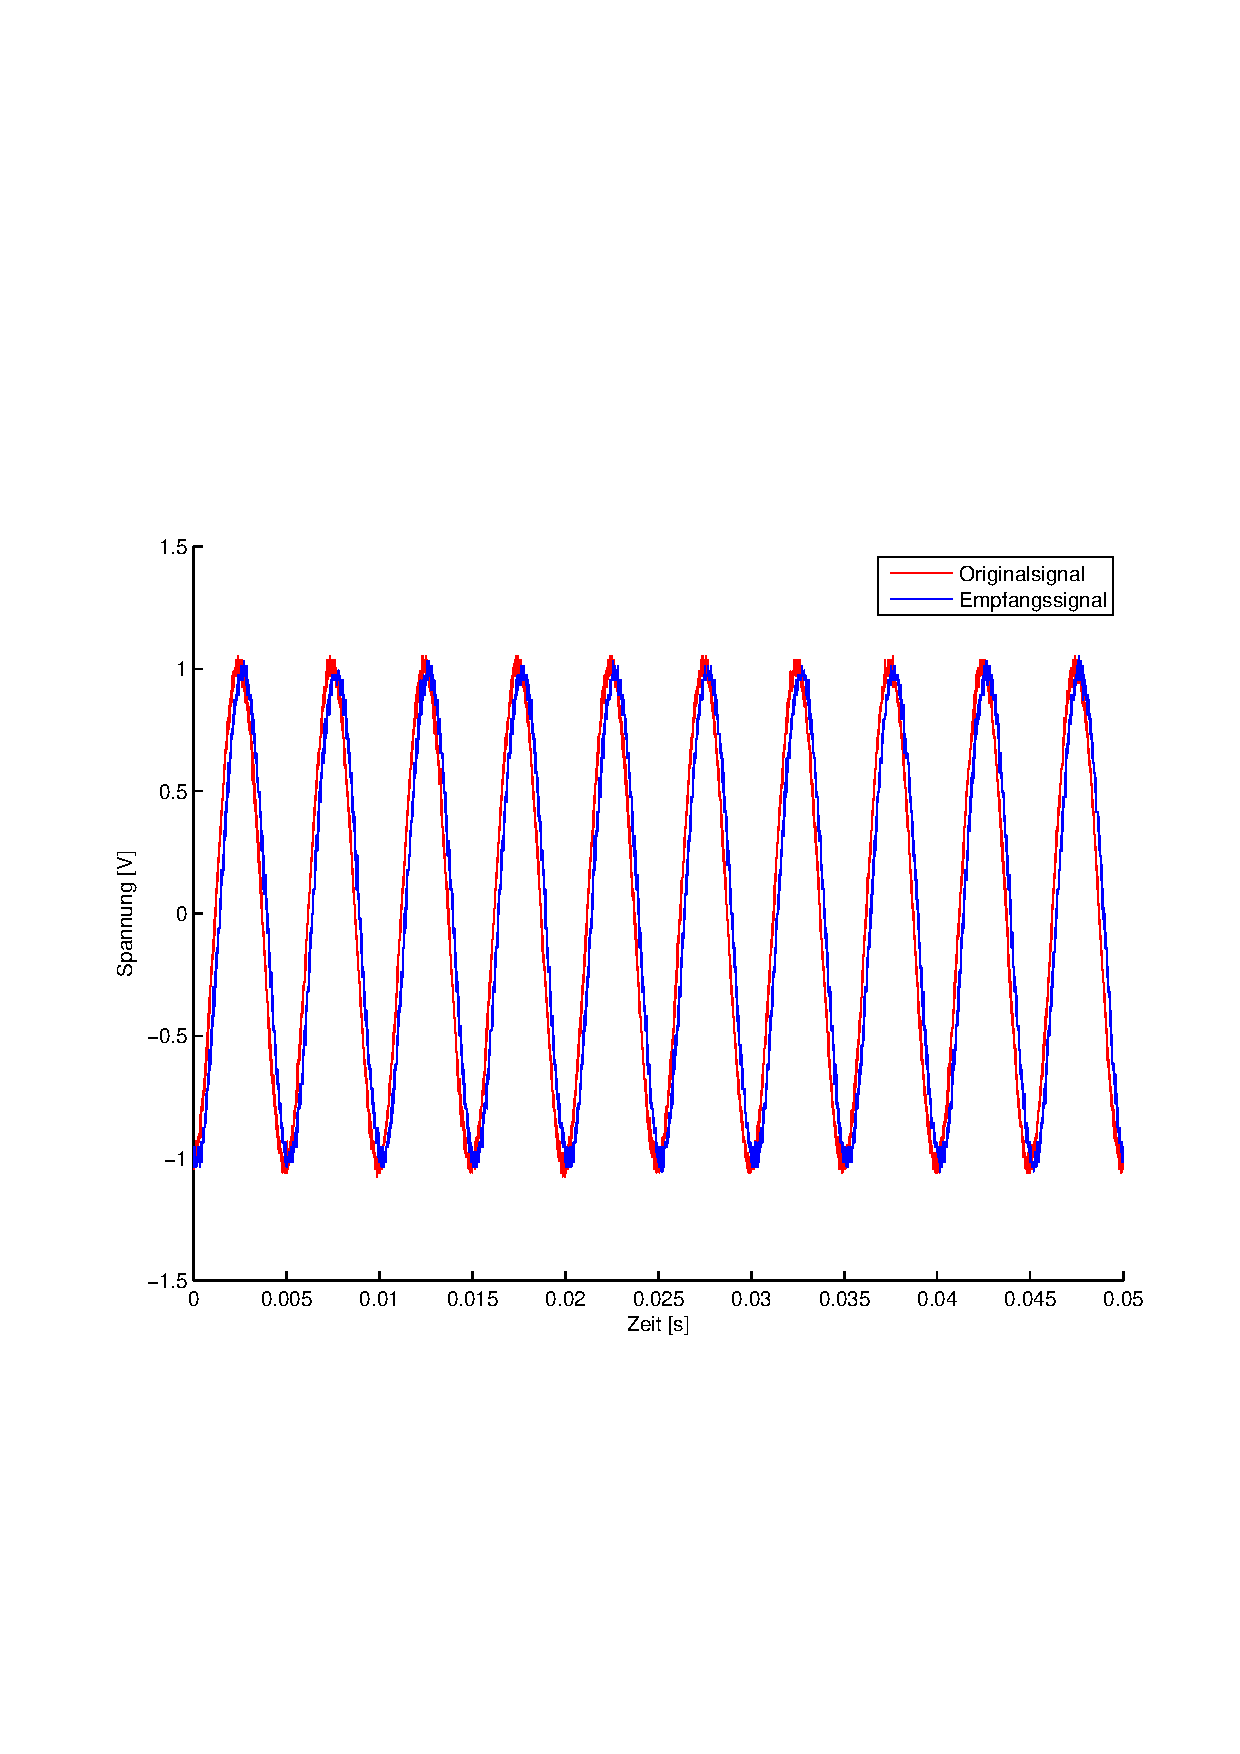
\includegraphics[scale=0.5, trim = 16mm 70mm 16mm 85mm, clip]
                                        {Bilder/100kHz_sin_Signal_Rekonstuiert}
                          \caption{100 kHz Sinus noch verschoben}
                          \label{fig:100kHz_sin_rek}
                    \end{figure}
                \end{minipage}
                
                \begin{minipage}{0.6\textwidth}
                    \begin{figure}[H]
                        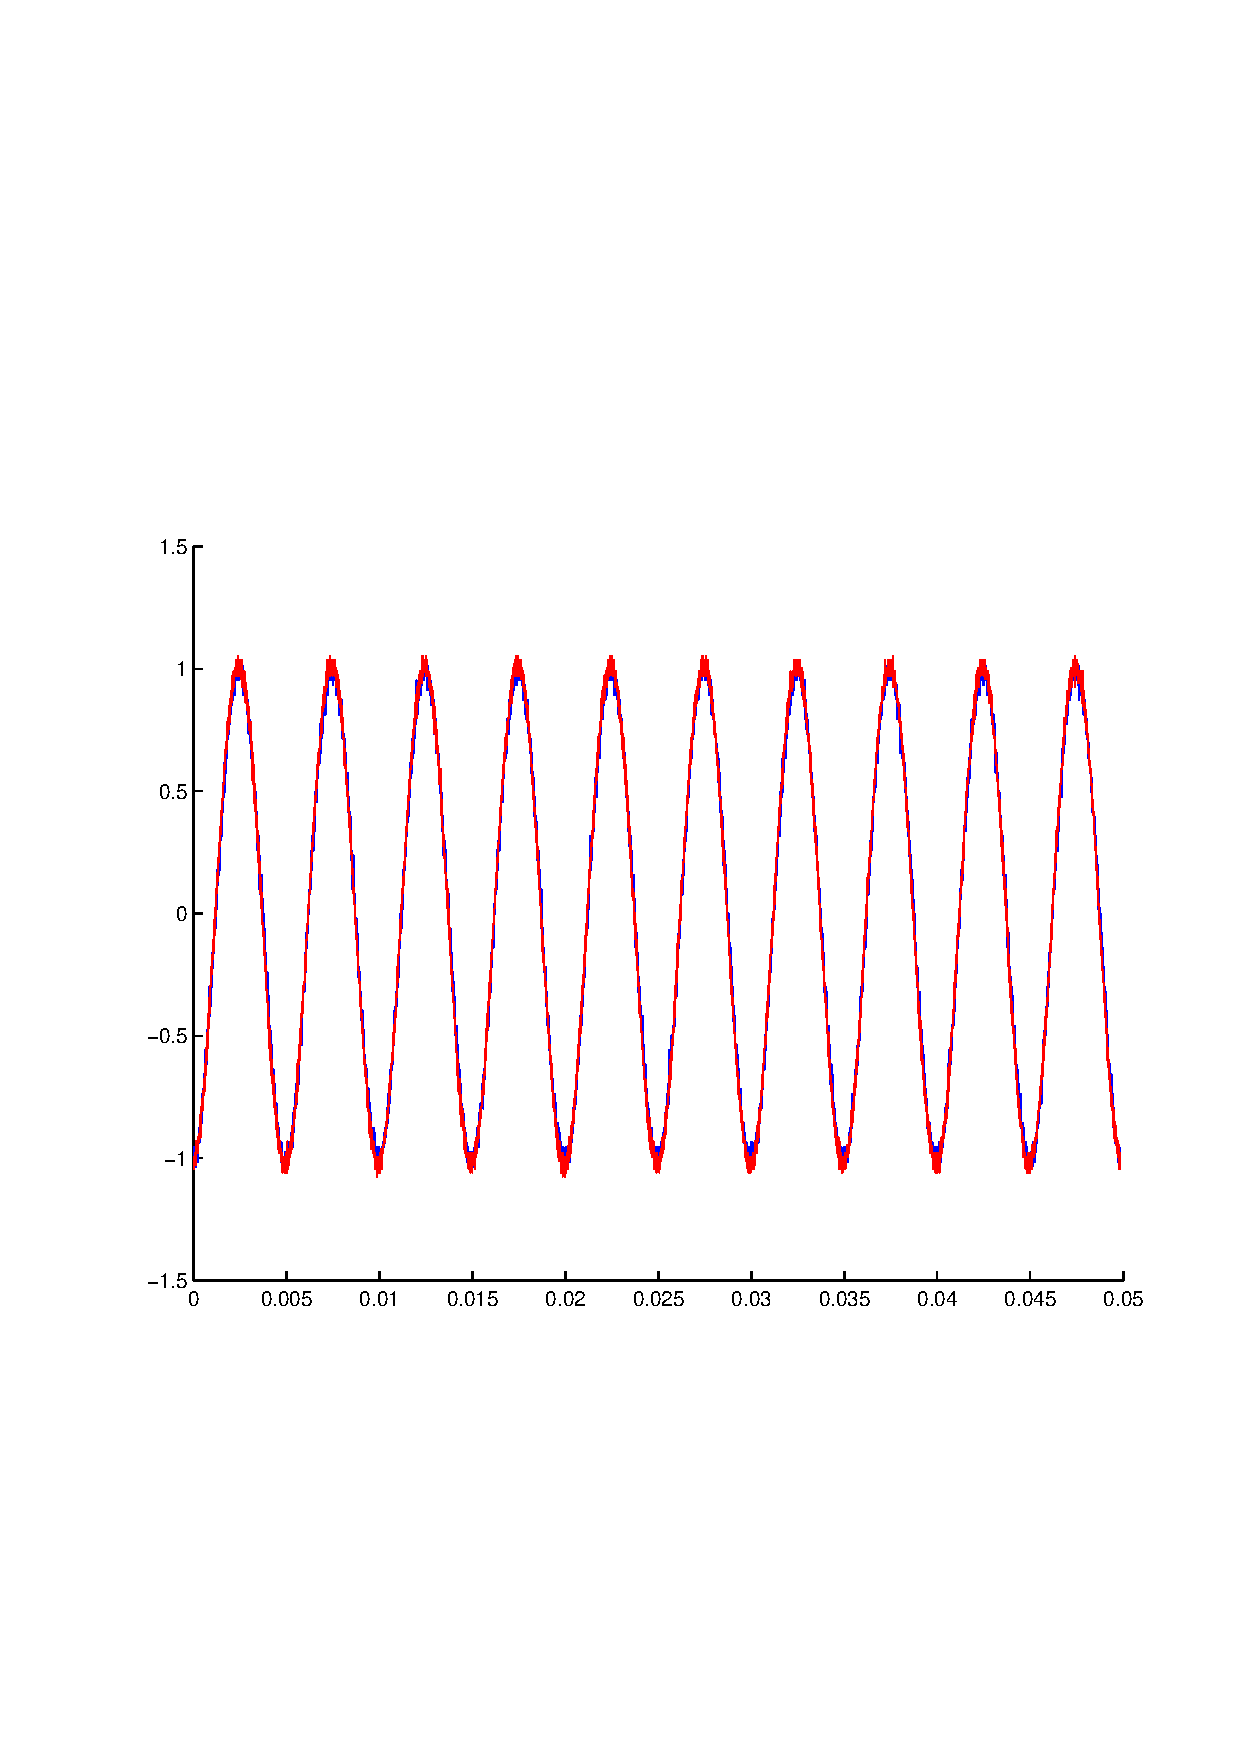
\includegraphics[scale=0.5, trim = 16mm 70mm 16mm 85mm, clip]
                                        {Bilder/100kHz_sin_Signal_Rekonstuiert_delayed}
                       \caption{100 kHz Sinus angepasst}
                      \label{fig:100kHz_sin_rek_angepasst}
                    \end{figure}
                \end{minipage}
            
            \end{tabular}
        \end{center}
        
        \vspace{2em}
        
        
        
        Anschließend können Sendesignal und dekodiertes Signal voneinander subrahiert werden und man erhält den
        Quantisierungsfehler. Die Quantisierungsfehler sind in den Abbildungen \ref{fig:QuantErr 100 kHz
        Sinus},\ref{fig:QuantErr 100 kHz Dreieck}, \ref{fig:QuantErr 8 kHz Sinus} und \ref{fig:QuantErr 8 kHz
        Dreieck} zu sehen.\\
        
        \begin{center}
            \begin{tabular}{ll}
            
            \hspace{-4cm}
                \begin{minipage}{0.6\textwidth}
                    \begin{figure}[H]
                        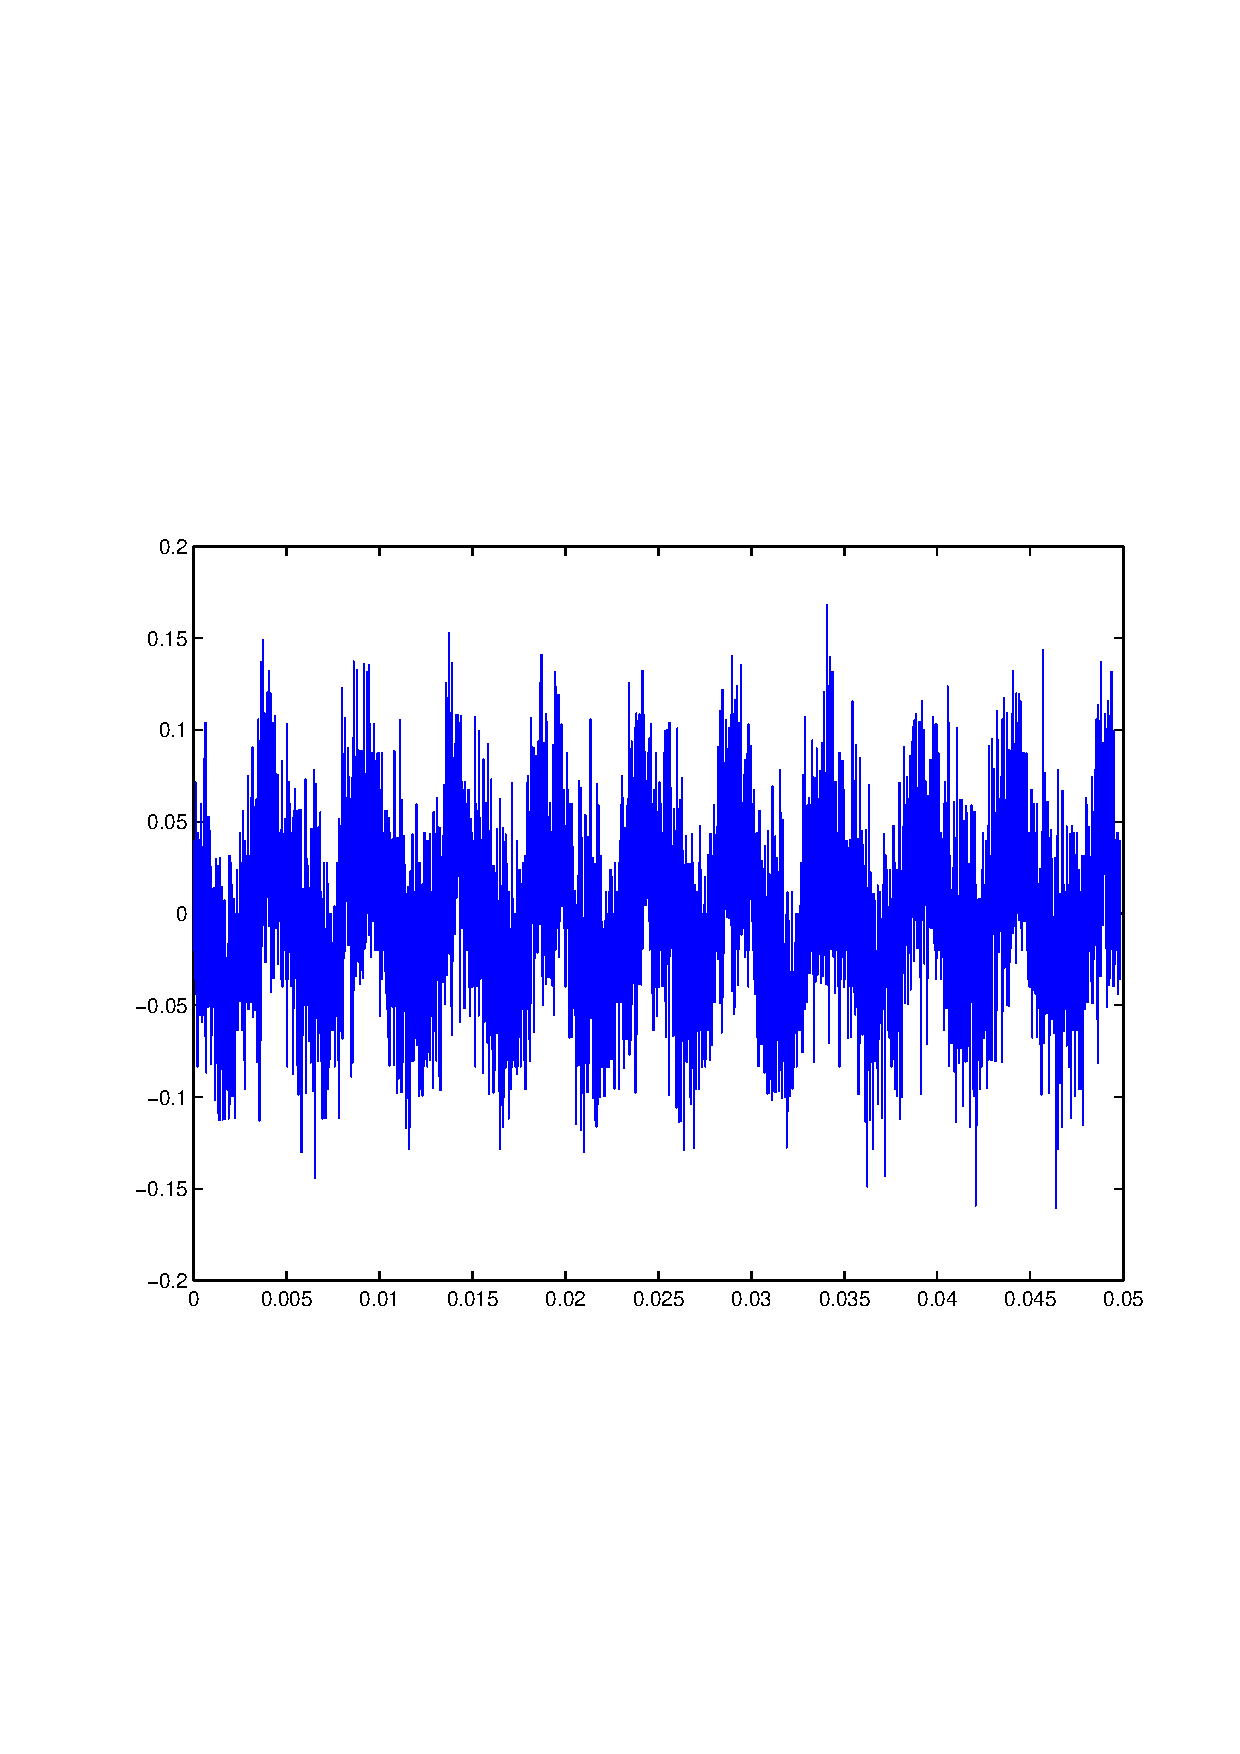
\includegraphics[scale=0.5, trim = 16mm 70mm 16mm 85mm, clip]
                                        {Bilder/100kHz_sin_Quantisierungsfehler}
                          \caption{Quantisierungsfehler 100 kHz Sinus}
                          \label{fig:QuantErr 100 kHz Sinus}
                    \end{figure}
                \end{minipage}
                
                \begin{minipage}{0.6\textwidth}
                    \begin{figure}[H]
                        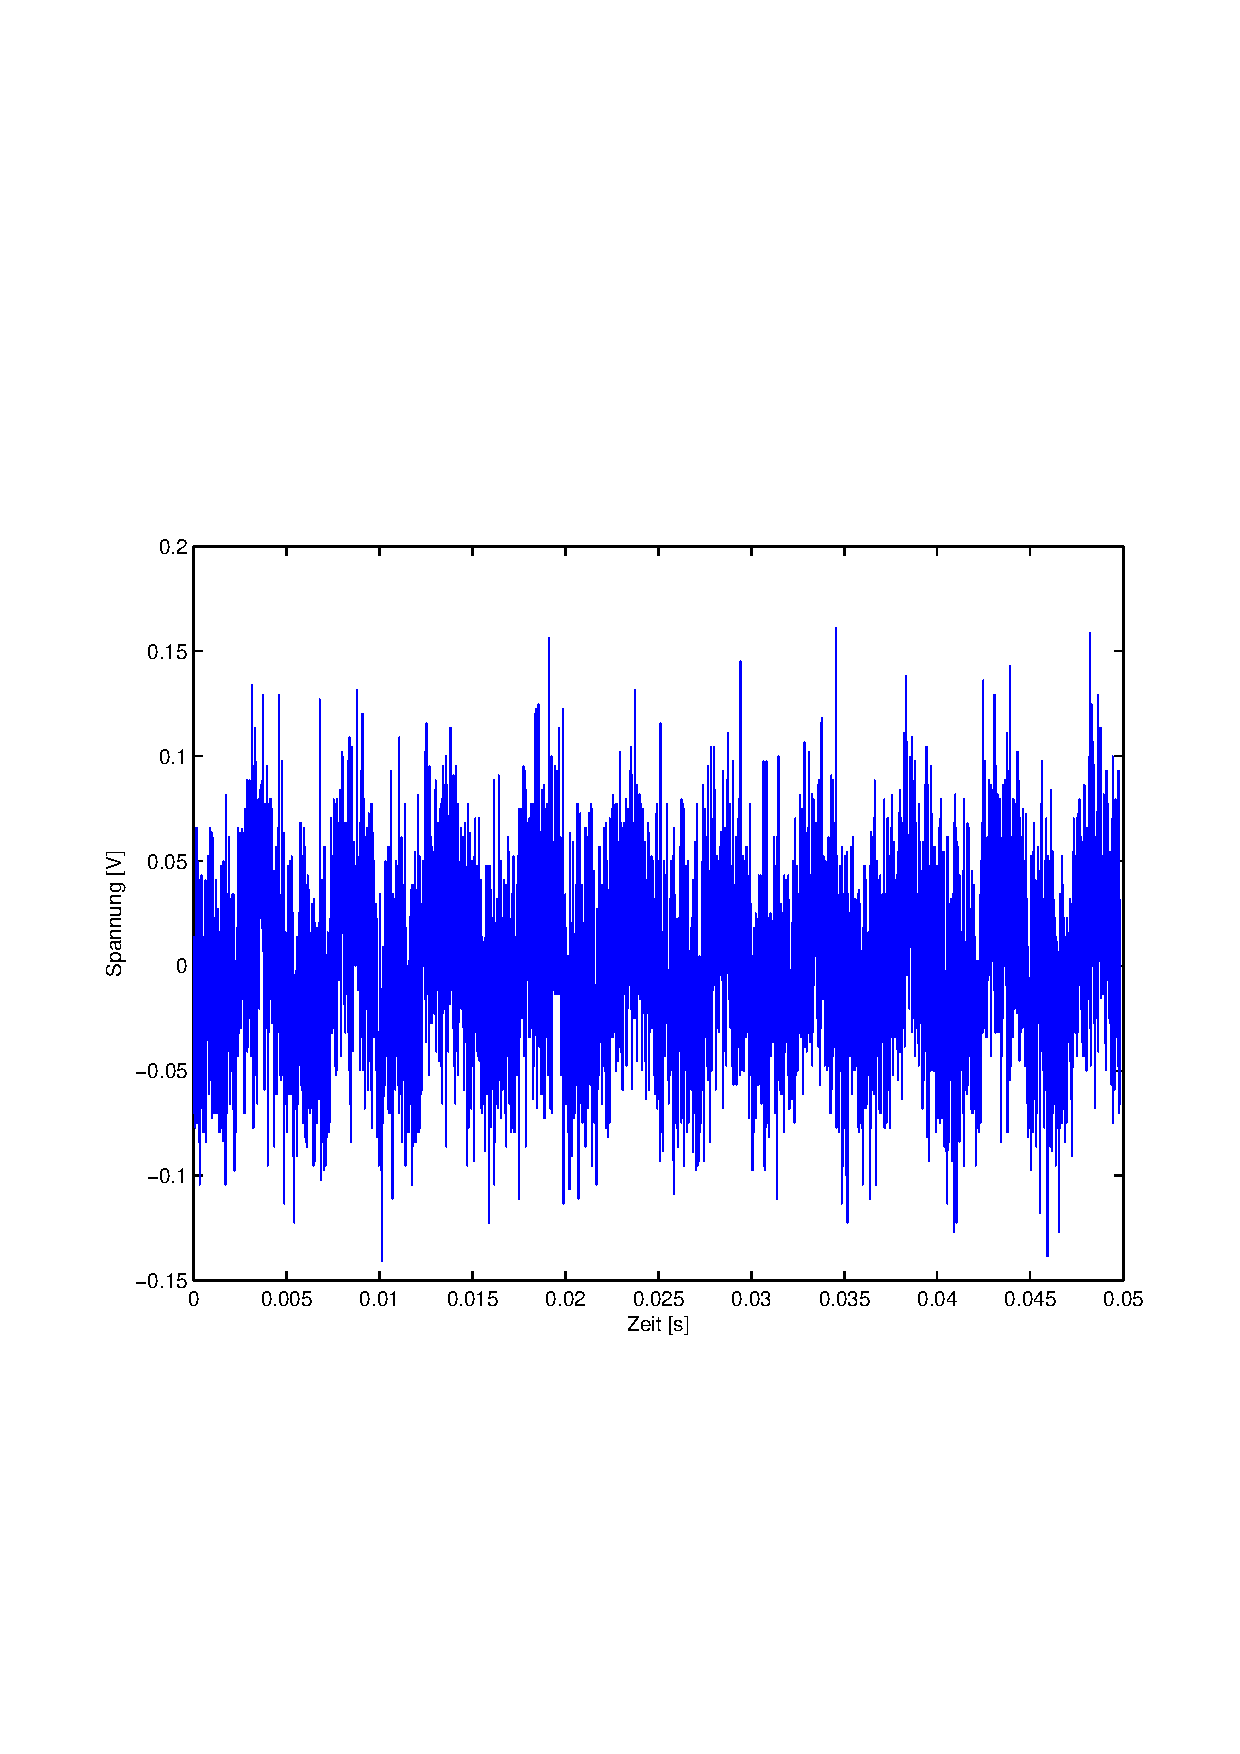
\includegraphics[scale=0.5, trim = 16mm 70mm 16mm 85mm, clip]
                                        {Bilder/100kHz_dreieck_Quantisierungsfehler}
                        \caption{Quantisierungsfehler 100 kHz Dreieck}
                        \label{fig:QuantErr 100 kHz Dreieck}
                    \end{figure}
                \end{minipage}
            
            \end{tabular}
        \end{center}
        
        
        
        \begin{center}
            \begin{tabular}{ll}
            
            \hspace{-4cm}
                \begin{minipage}{0.6\textwidth}
                    \begin{figure}[H]
                        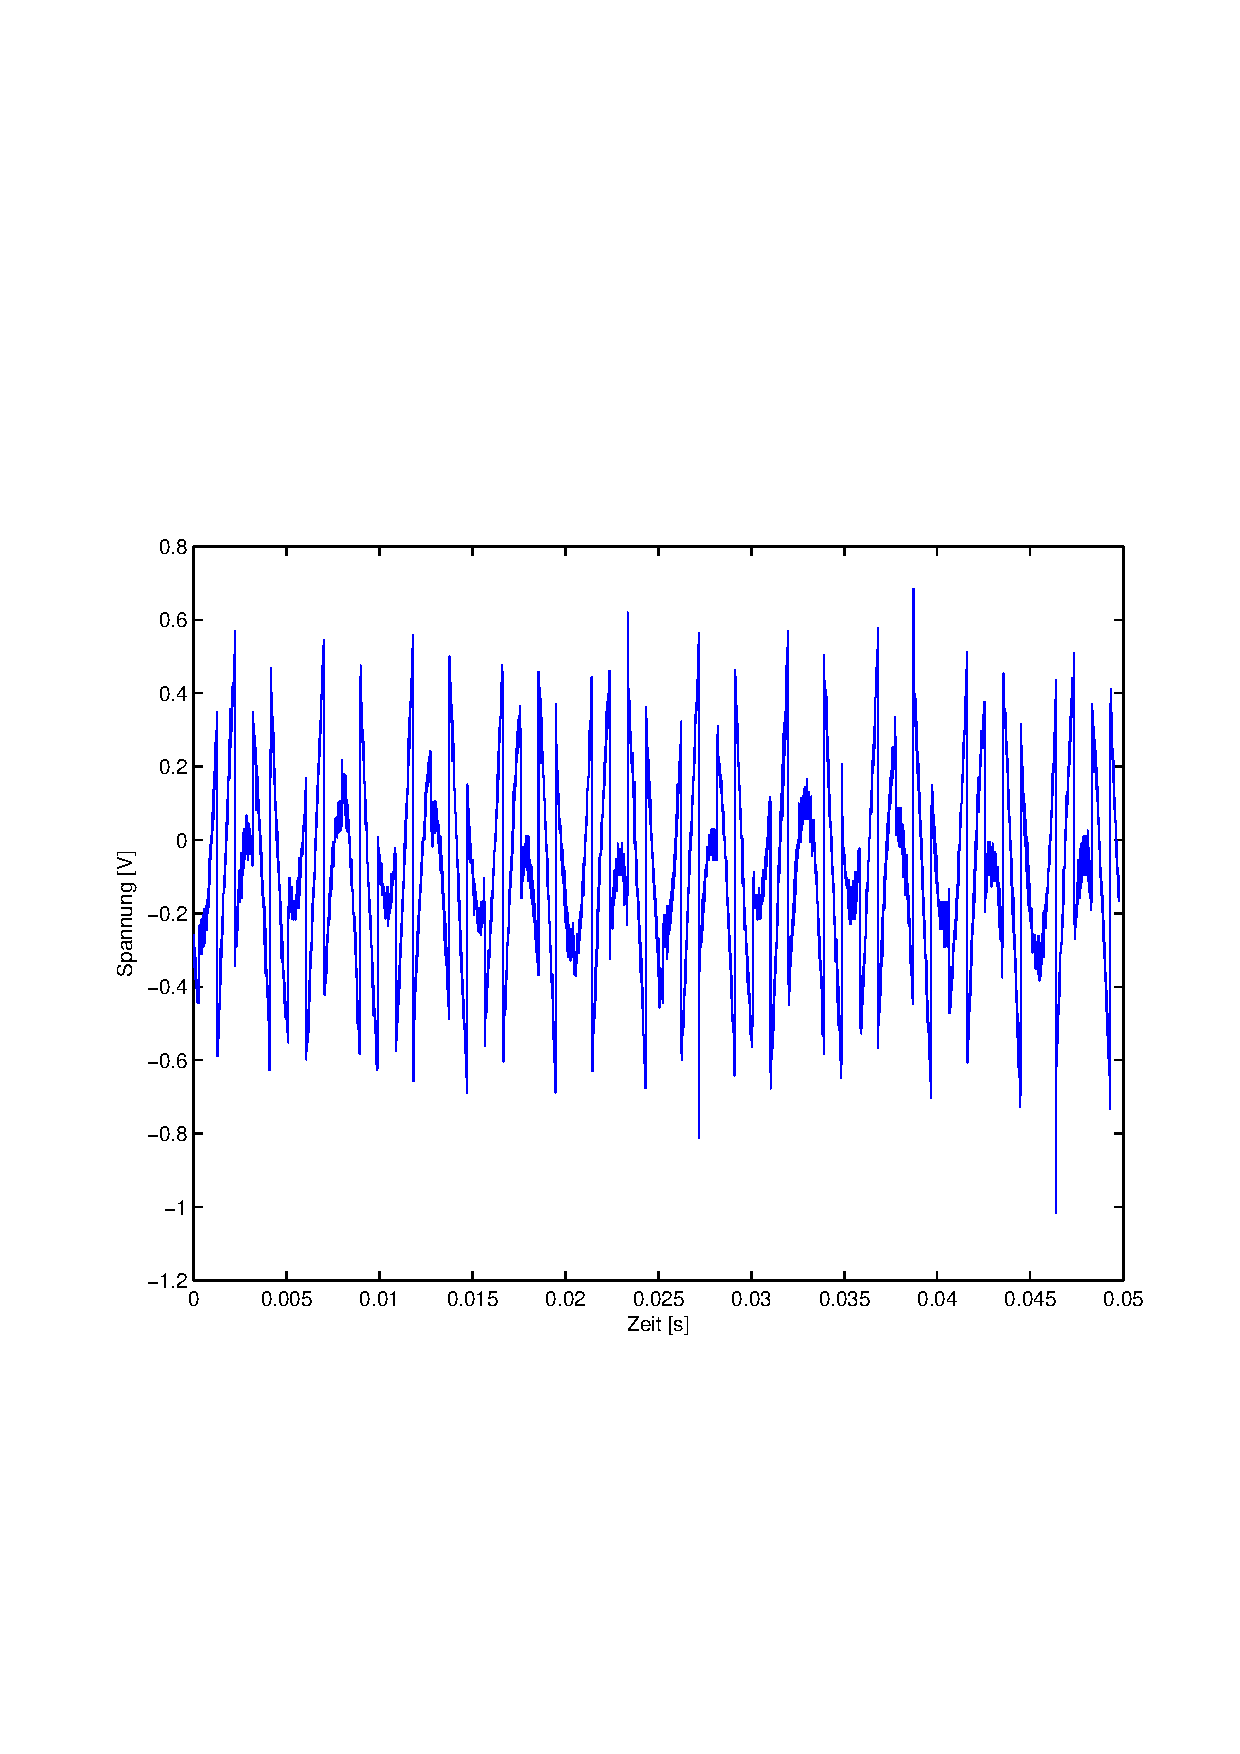
\includegraphics[scale=0.5, trim = 16mm 70mm 16mm 85mm, clip]
                                        {Bilder/8kHz_sin_Quantisierungsfehler}
                          \caption{Quantisierungsfehler 8 kHz Sinus}
                          \label{fig:QuantErr 8 kHz Sinus}
                    \end{figure}
                \end{minipage}
                
                \begin{minipage}{0.6\textwidth}
                    \begin{figure}[H]
                        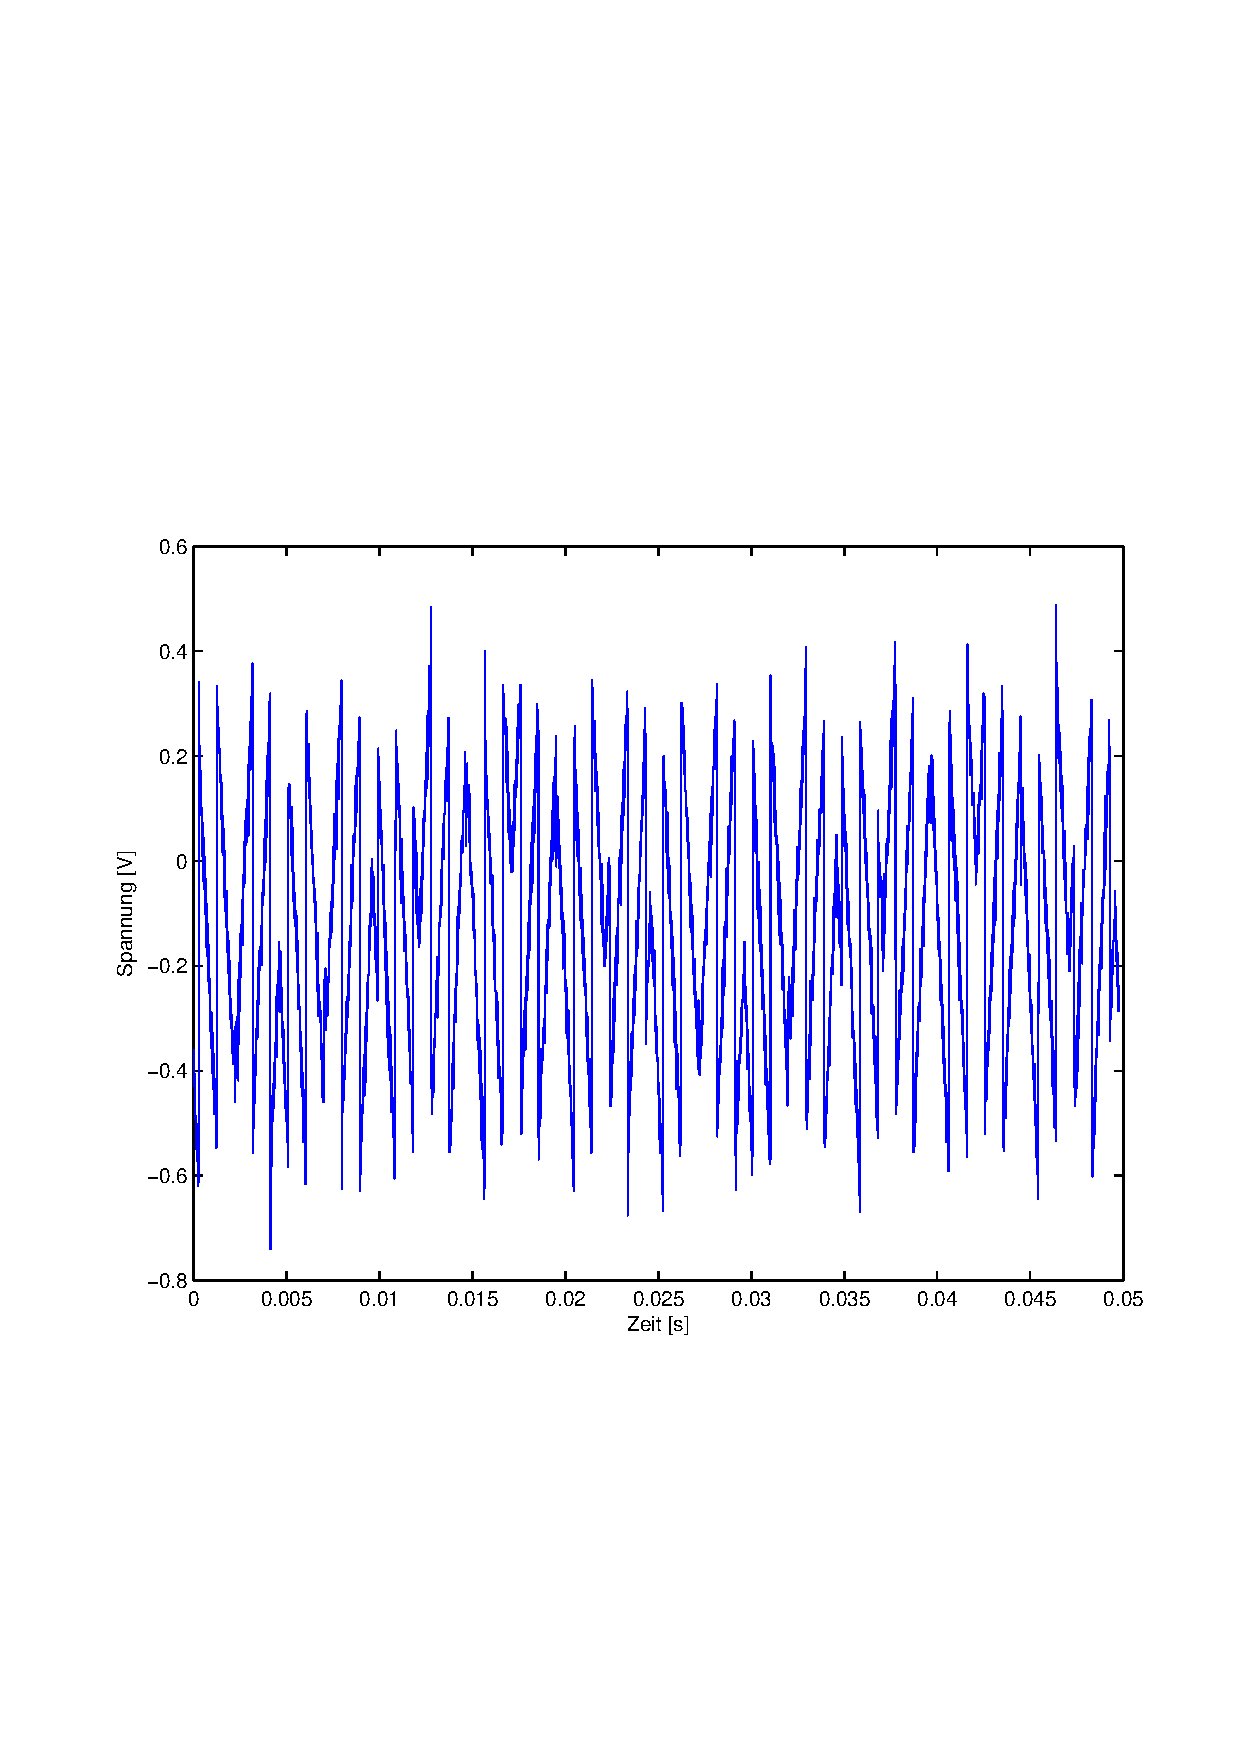
\includegraphics[scale=0.5, trim = 16mm 70mm 16mm 85mm, clip]
                                        {Bilder/8kHz_dreieck_Quantisierungsfehler}
                        \caption{Quantisierungsfehler 8 kHz Dreieck}
                        \label{fig:QuantErr 8 kHz Dreieck}
                    \end{figure}
                \end{minipage}
            
            \end{tabular}
        \end{center}
        \vspace{2em}
        
        Es ist gut zu erkennen, dass wie zu erwarten für die Abtastung mit 8 kHz ein von der Amplitude her wesentlich
        größerer Fehler auftritt als bei 100 kHz.
         
        \vspace{2em} 
         
        Mit dem Matlabbefehl hist wird der Quantisierungsfehler als Häufigkeitsverteilung geplottet. Die Ergebnisse sind in
        Abbildung \ref{fig:100kHz_drei_Hist}, \ref{fig:100kHz_sin_Hist}, \ref{fig:8kHz_drei_Hist} und
        \ref{fig:8kHz_sin_Hist} zu sehen.
        
        \begin{center}
            \begin{tabular}{ll}
            
            \hspace{-4cm}
                \begin{minipage}{0.6\textwidth}
                    \begin{figure}[H]
                        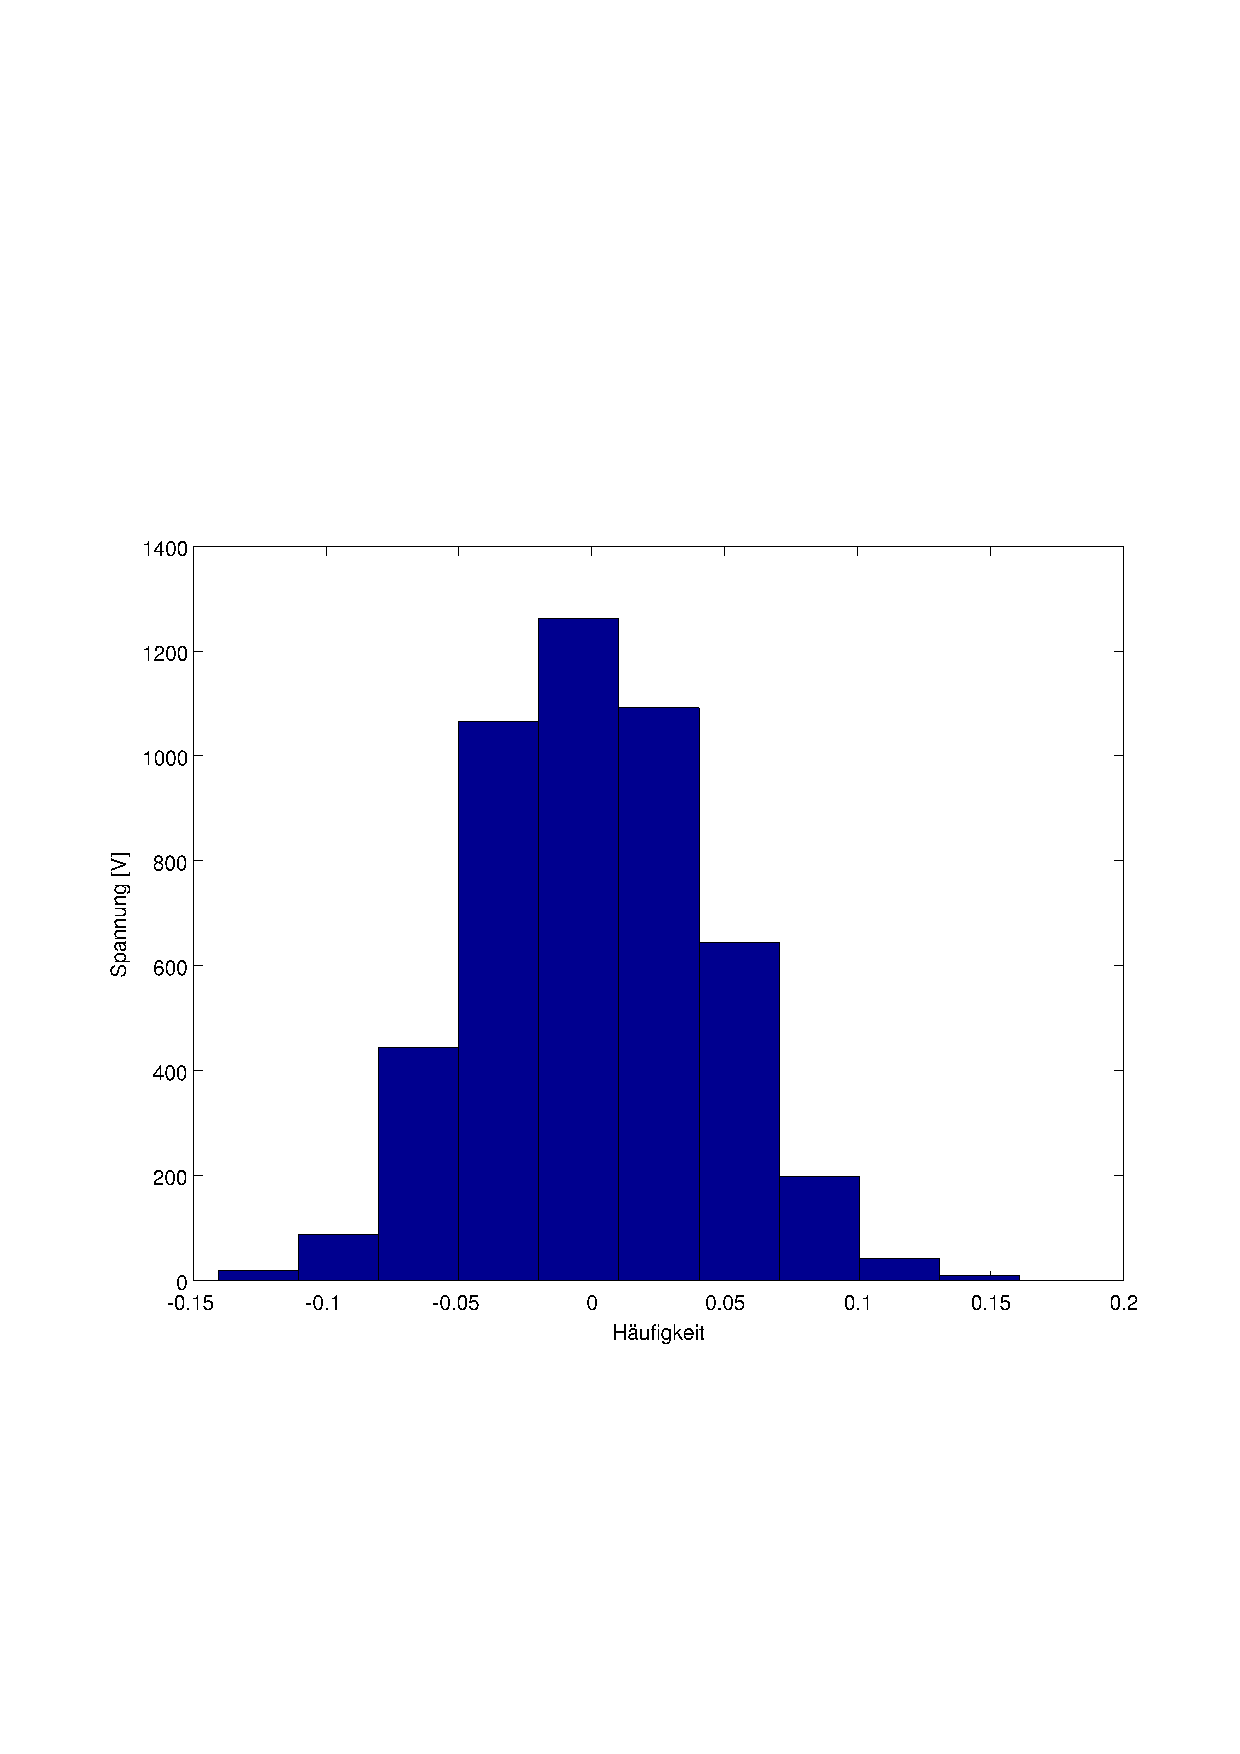
\includegraphics[scale=0.5, trim = 16mm 70mm 16mm 85mm, clip]
                                        {Bilder/100kHz_dreieck_Quant_Hist}
                        \caption{100 kHz Dreieck Quantisierungsfehler Histplot}
                        \label{fig:100kHz_drei_Hist}
                    \end{figure}
                \end{minipage}
                
                \begin{minipage}{0.6\textwidth}
                    \begin{figure}[H]
                        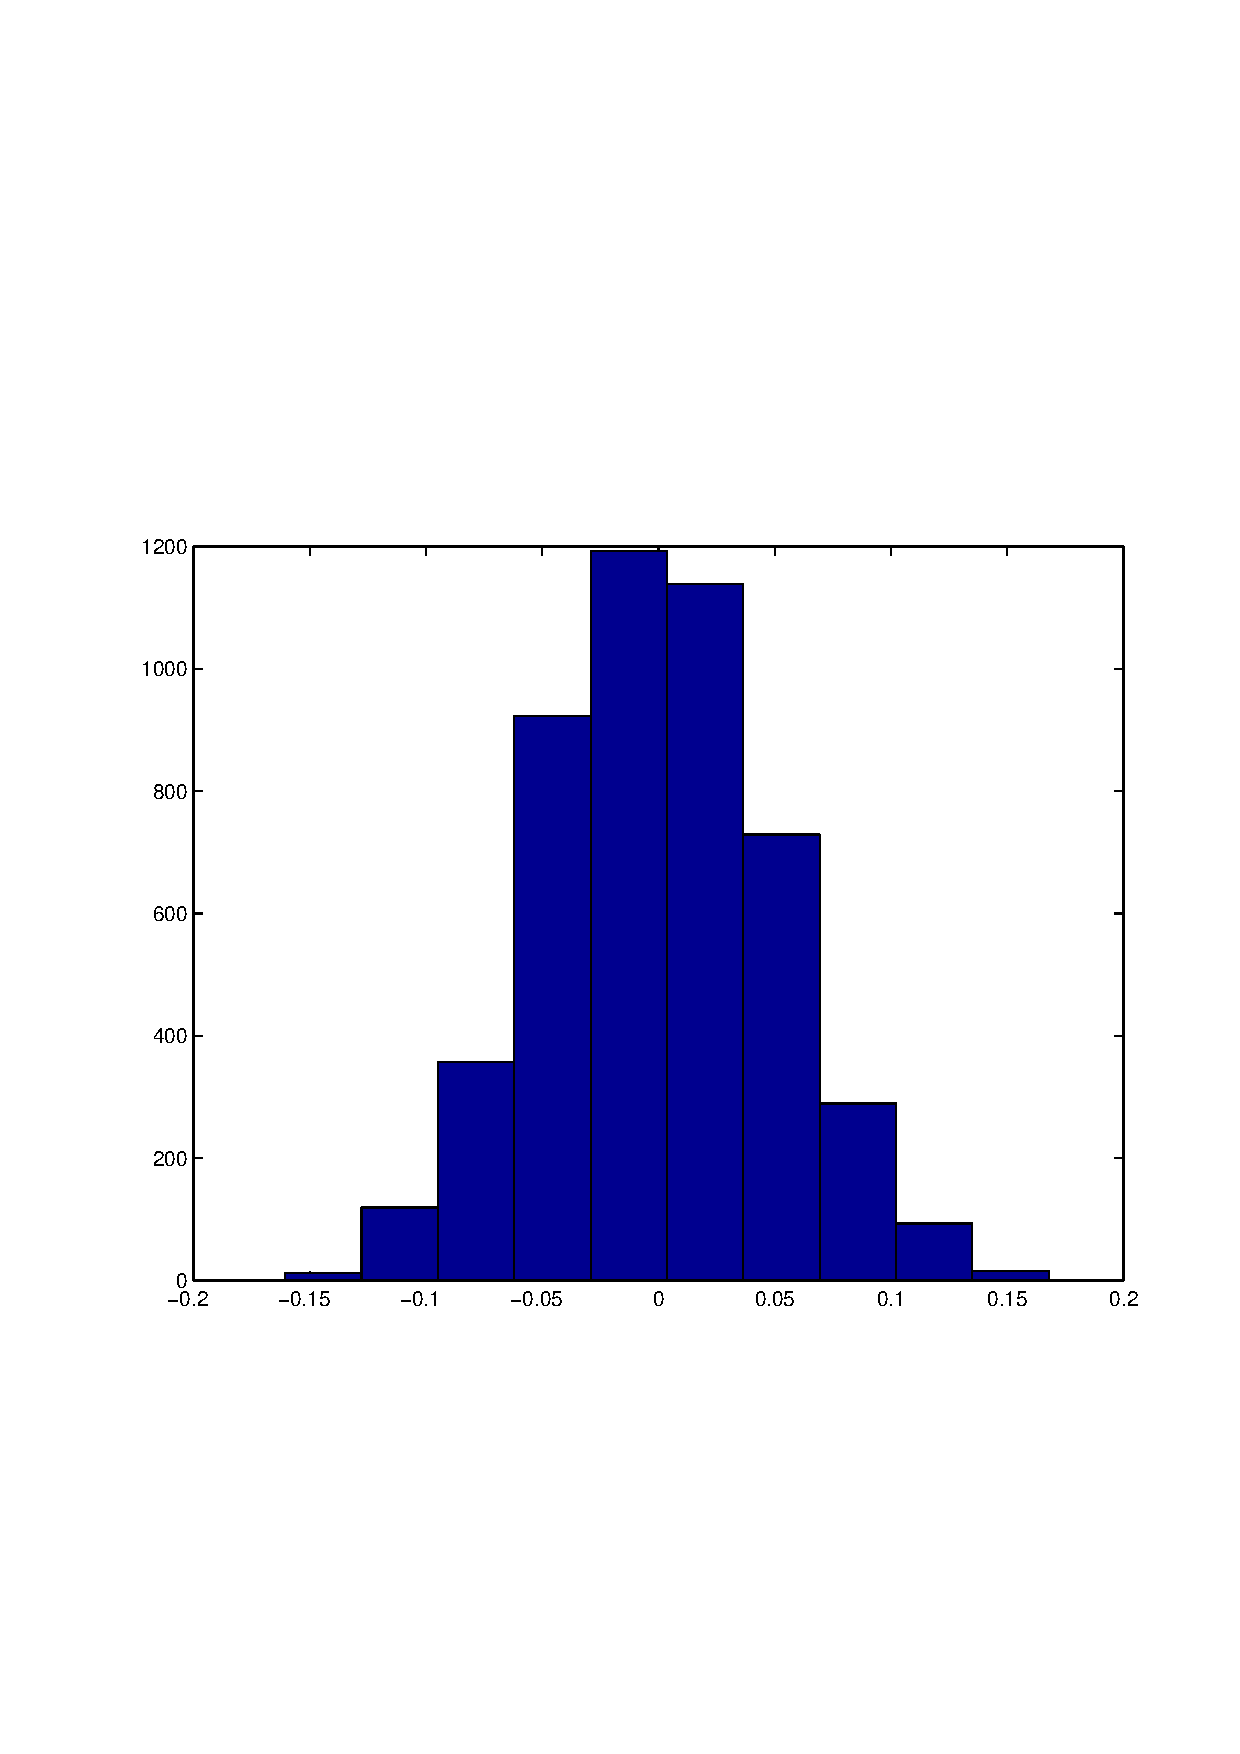
\includegraphics[scale=0.5, trim = 16mm 70mm 16mm 85mm, clip]
                                        {Bilder/100kHz_sin_Quant_Hist}
                        \caption{100 kHz Sinus Quantisierungsfehler Histplot}
                        \label{fig:100kHz_sin_Hist}
                    \end{figure}
                \end{minipage}
            
            \end{tabular}
        \end{center}
        
        
        
        \begin{center}
            \begin{tabular}{ll}
            
            \hspace{-4cm}
                \begin{minipage}{0.6\textwidth}
                    \begin{figure}[H]
                        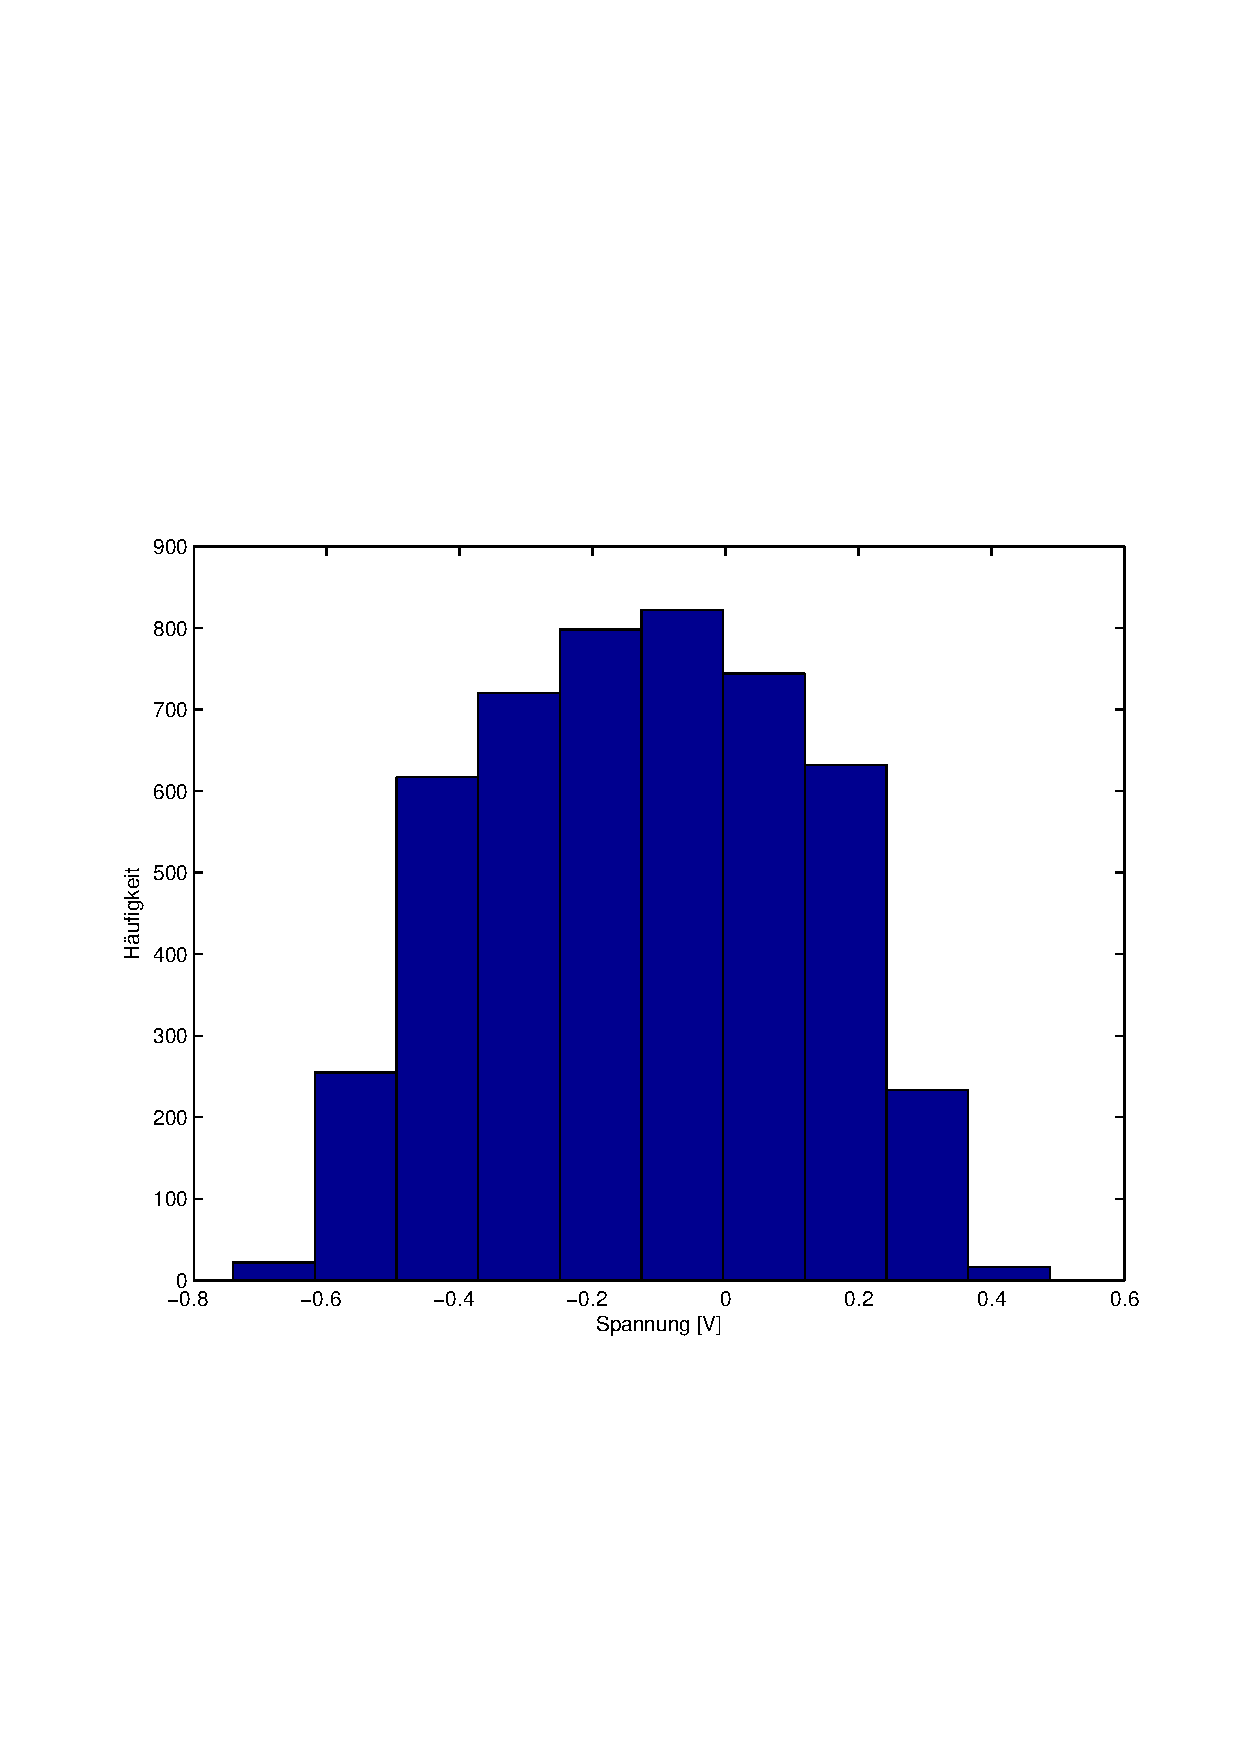
\includegraphics[scale=0.5, trim = 16mm 70mm 16mm 85mm, clip]
                                        {Bilder/8kHz_dreieck_Quant_Hist}
                        \caption{8 kHz Dreieck Quantisierungsfehler Histplot}
                        \label{fig:8kHz_drei_Hist}
                    \end{figure}
                \end{minipage}
                
                \begin{minipage}{0.6\textwidth}
                    \begin{figure}[H]
                        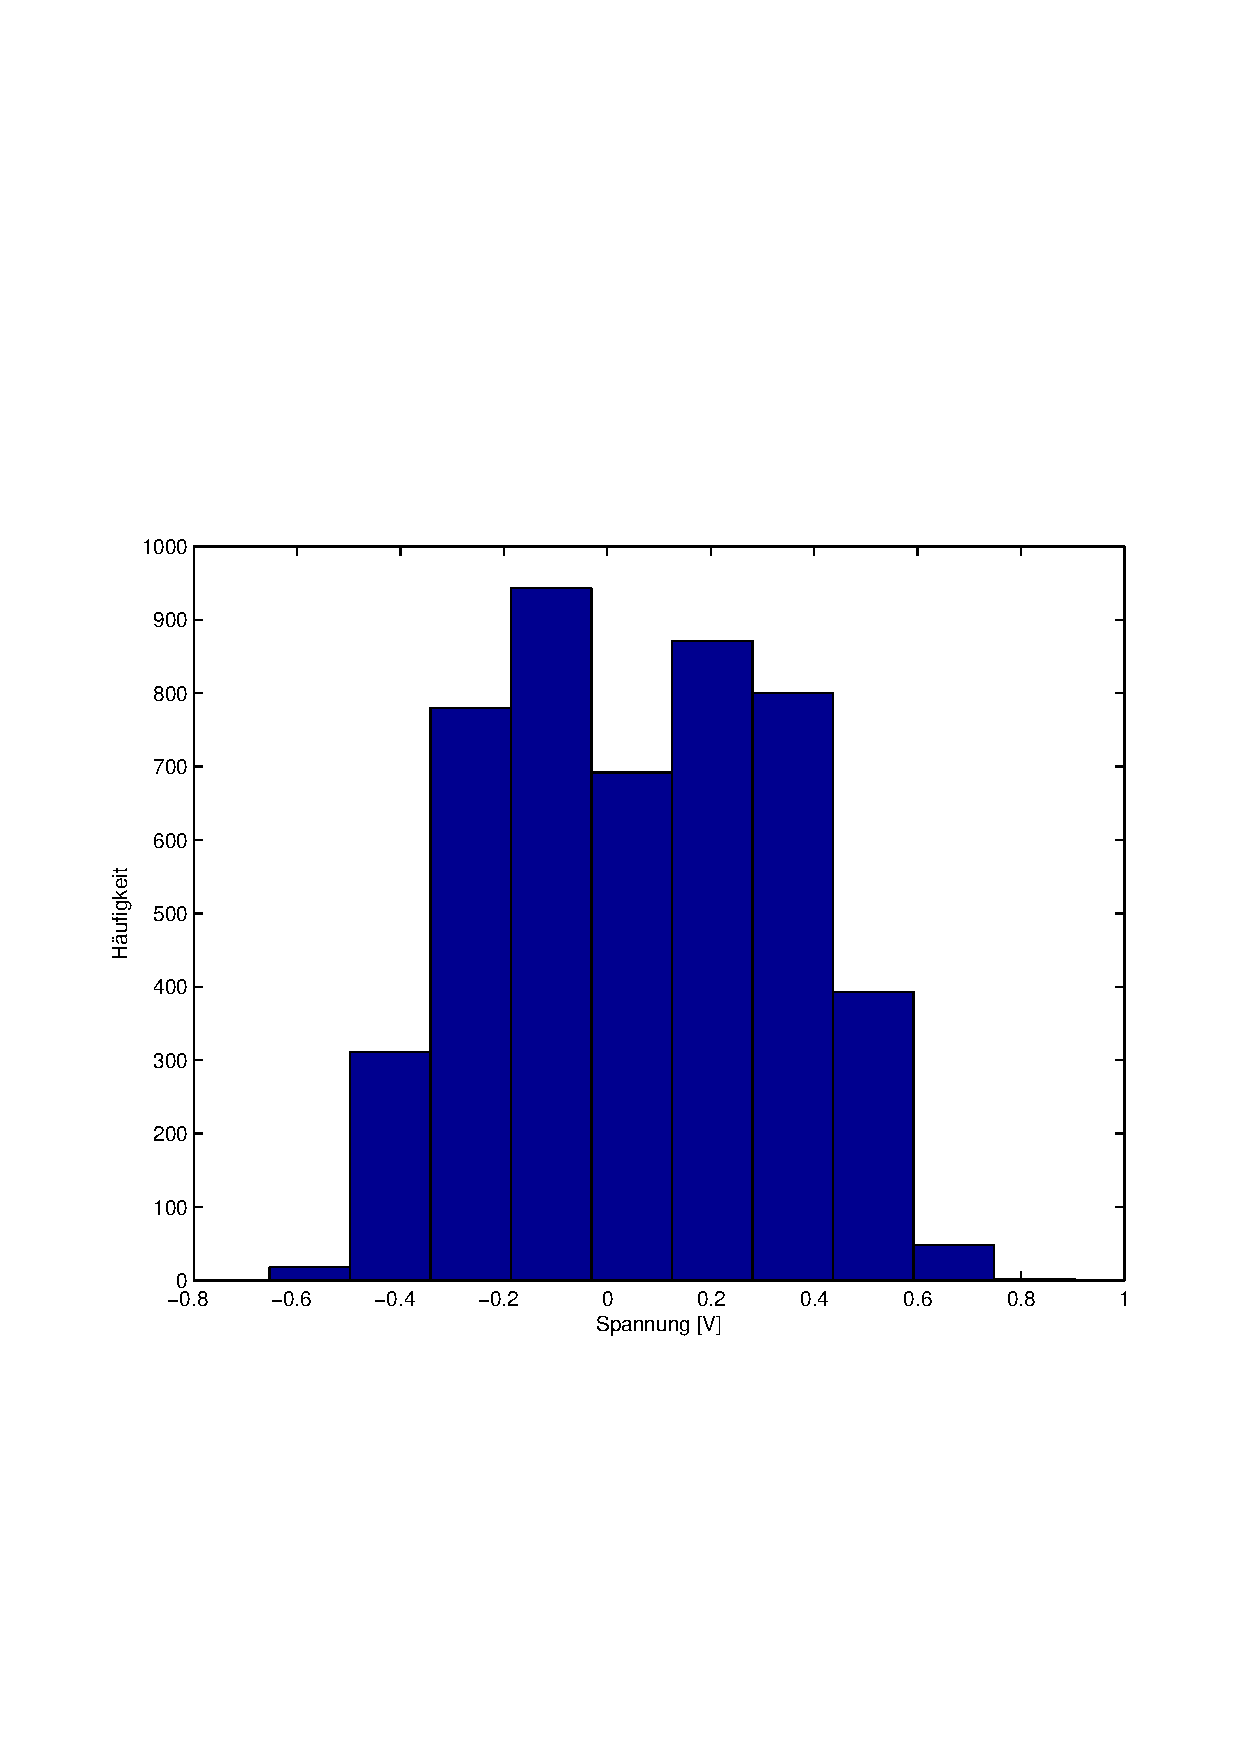
\includegraphics[scale=0.5, trim = 16mm 70mm 16mm 85mm, clip]
                                        {Bilder/8kHz_sin_Quant_Hist}
                        \caption{8 kHz Sinus Quantisierungsfehler Histplot}
                        \label{fig:8kHz_sin_Hist}
                    \end{figure}
                \end{minipage}
            
            \end{tabular}
        \end{center}
        
        \vspace{2em}
        
        Der Quantisierungsfehler, bzw. das Quantisierungsrauschen ist wie erwartet gaußverteilt.
        In den Histplots ist auch zu erkennen, dass bei der Abtastung mit 100 kHz die Amplituden des
        Quantisierungsfehlers geringer ist als bei der mit 8 kHz. Des weiteren treten die kleinen Fehler um die 0
        wesentlich häufiger auf und es ergibt sich eine schmalere Gaußverteilung.
         
        \vspace{2em}
        
        Für das Leistungsdichtespektrum wird die Autokorrelation des Quantisierungsfehlers mit dem Befehl xcorr aus
        Matlab gebildet und das Ergebnis dann fouriertransformiert (Abb. \ref{fig:100kHz_drei_LDS} und
        \ref{fig:100kHz_sin_LDS}).
        
        \begin{center}
            \begin{tabular}{ll}
            
            \hspace{-4cm}
                \begin{minipage}{0.6\textwidth}
                    \begin{figure}[H]
                        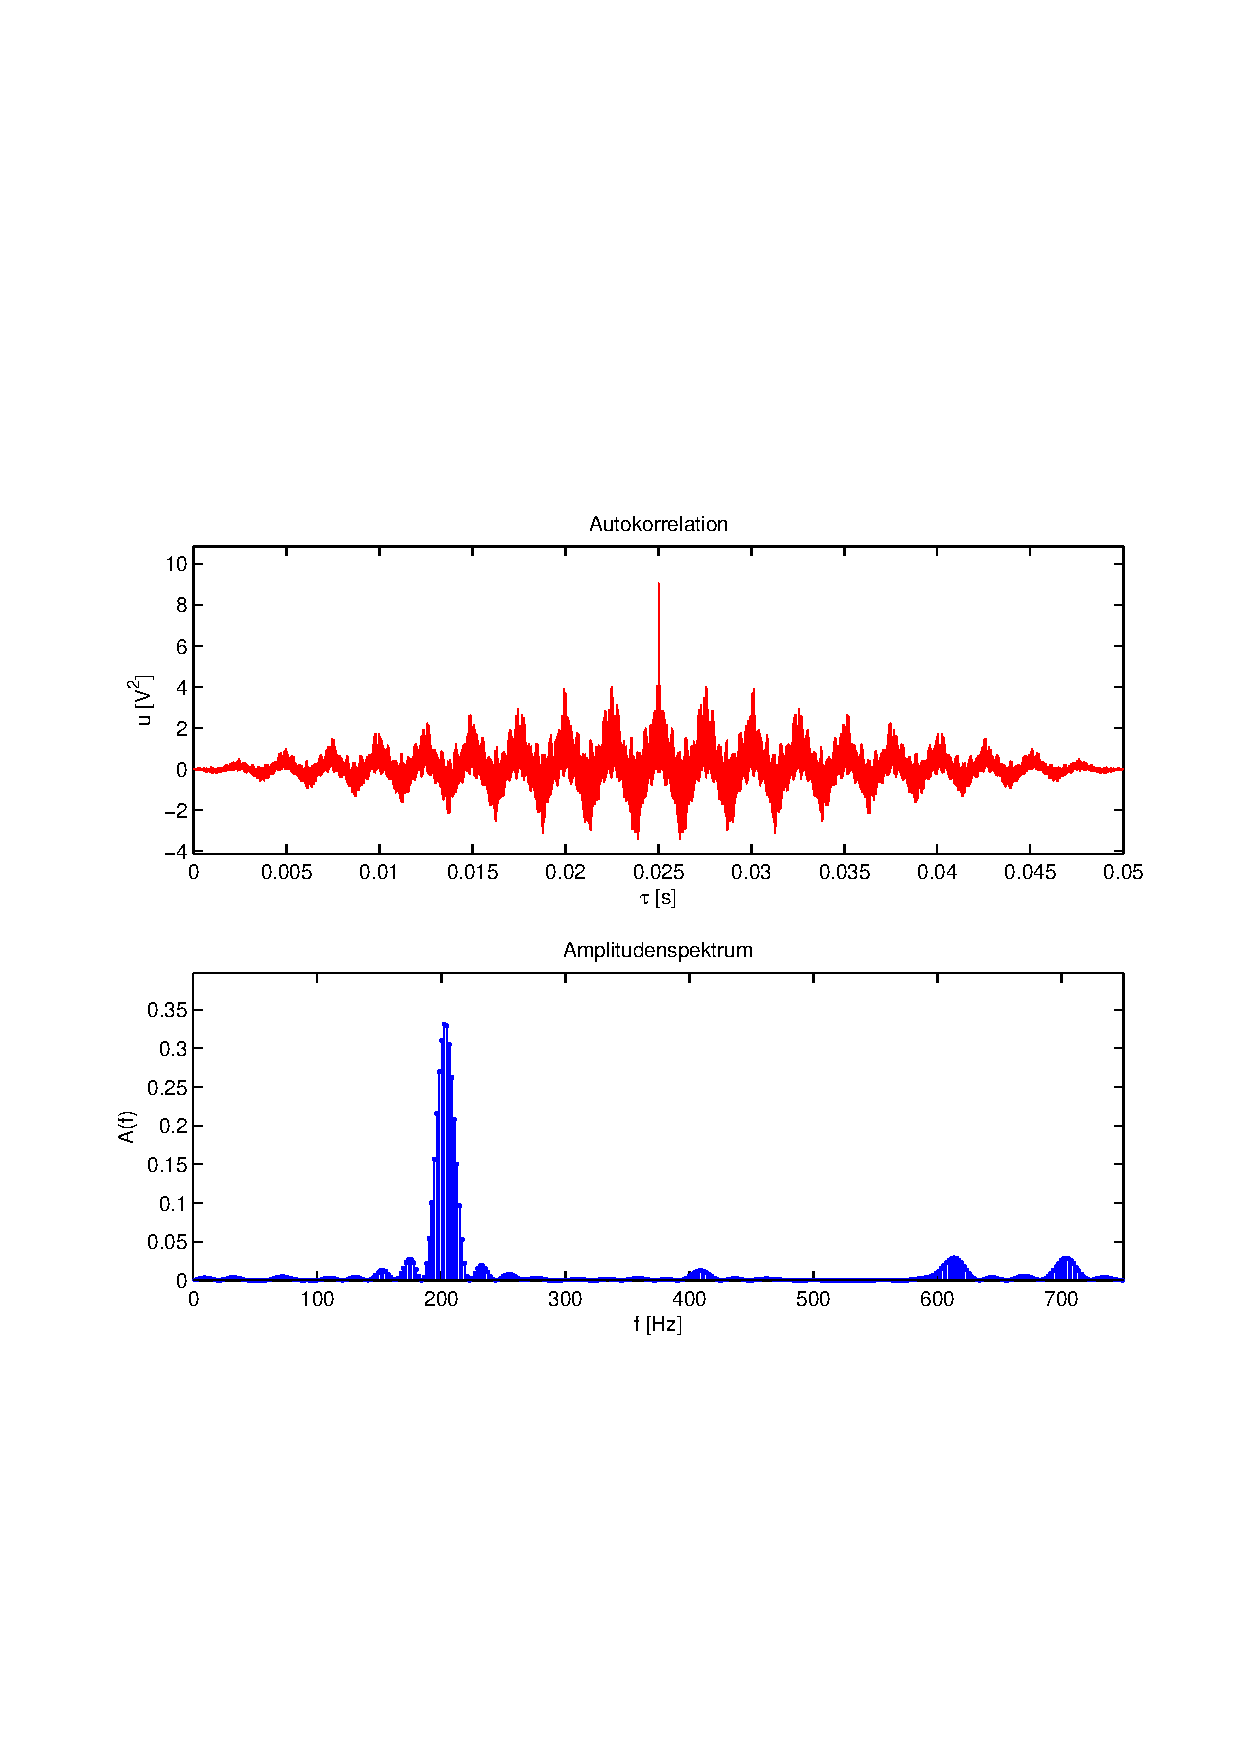
\includegraphics[scale=0.5, trim = 16mm 70mm 16mm 85mm, clip]
                                        {Bilder/100kHz_dreieck_LSD}
                        \caption{100 kHz Dreieck Quantisierungsfehler LDS}
                        \label{fig:100kHz_drei_LDS}
                    \end{figure}
                \end{minipage}
                
                \begin{minipage}{0.6\textwidth}
                    \begin{figure}[H]
                        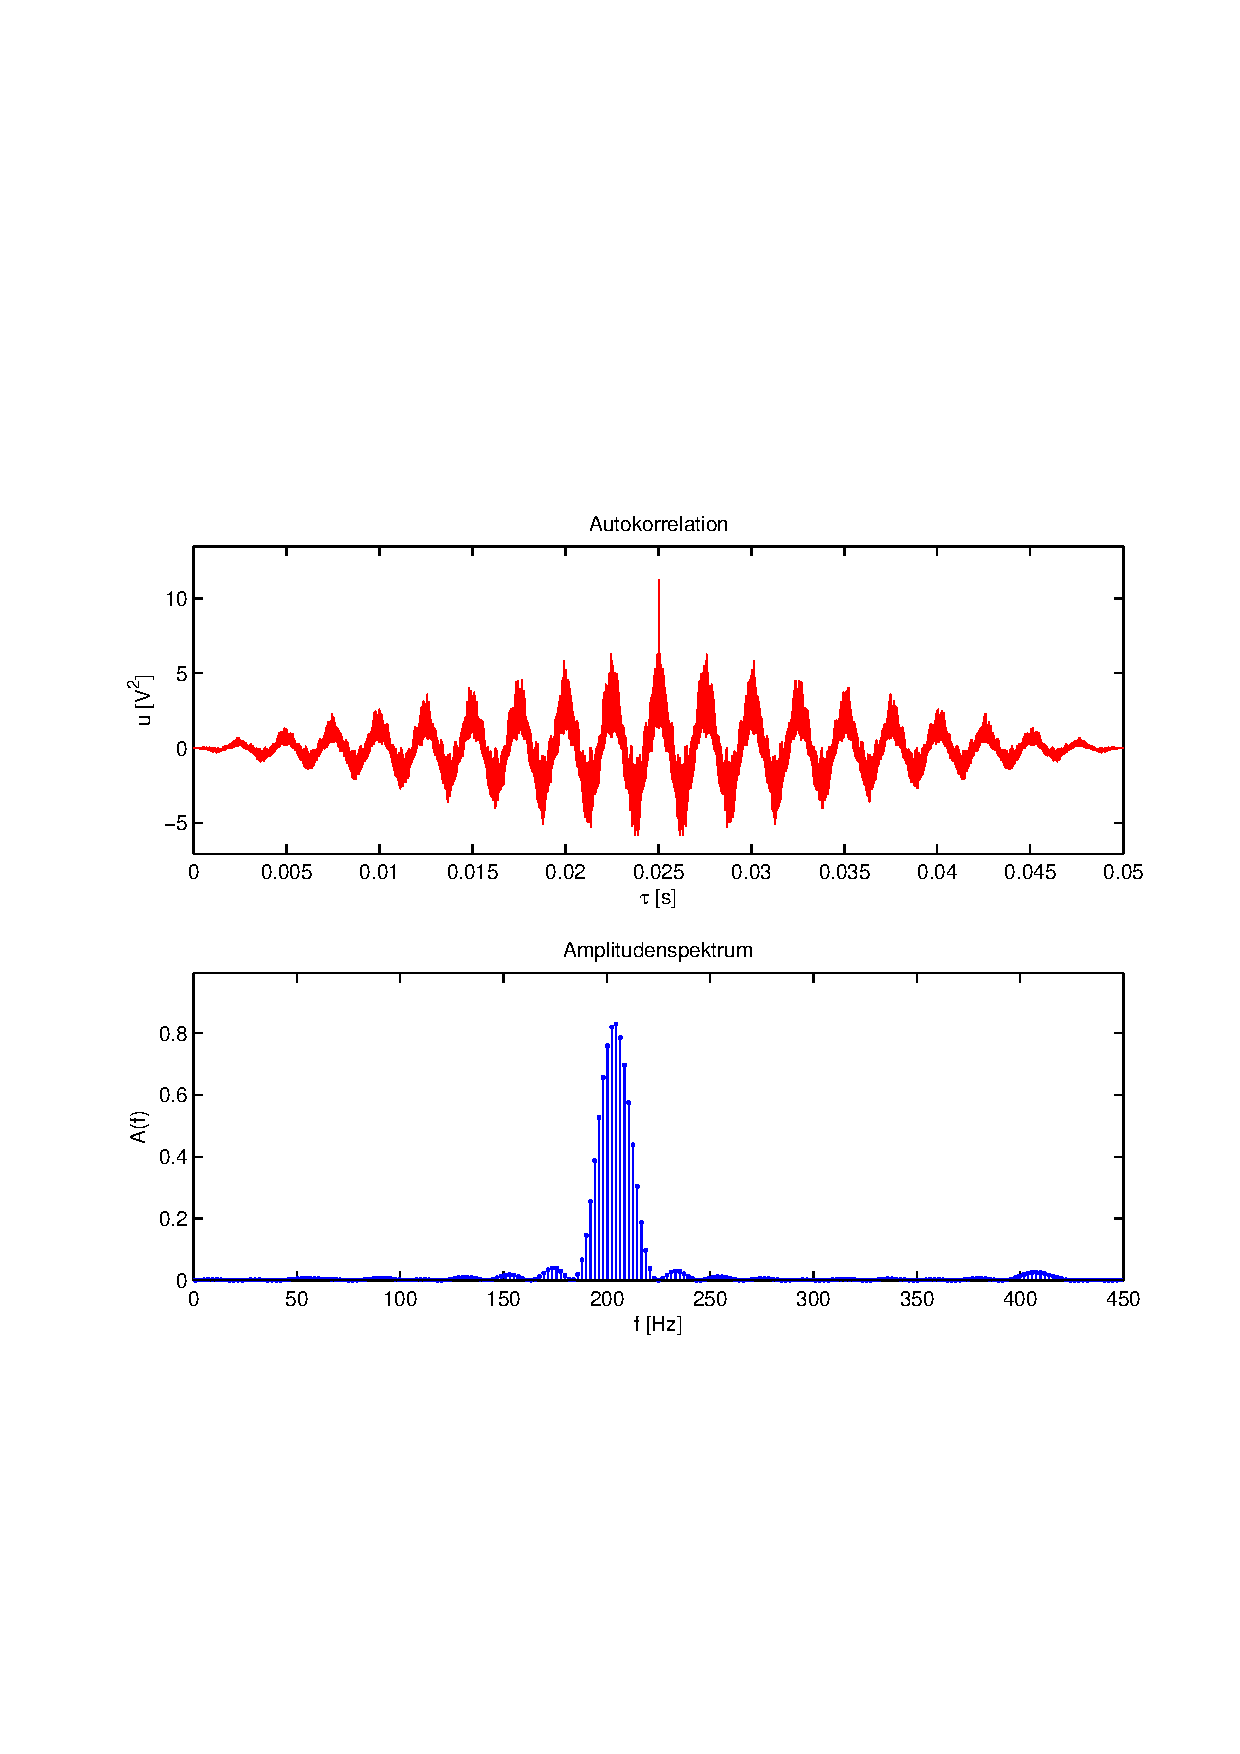
\includegraphics[scale=0.5, trim = 16mm 70mm 16mm 85mm, clip]
                                        {Bilder/100kHz_sin_LSD}
                        \caption{100 kHz Sinus Quantisierungsfehler LDS}
                        \label{fig:100kHz_sin_LDS}
                    \end{figure}
                \end{minipage}
            
            \end{tabular}
        \end{center}
        
        
        
        \begin{center}
            \begin{tabular}{ll}
            
            \hspace{-4cm}
                \begin{minipage}{0.6\textwidth}
                    \begin{figure}[H]
                        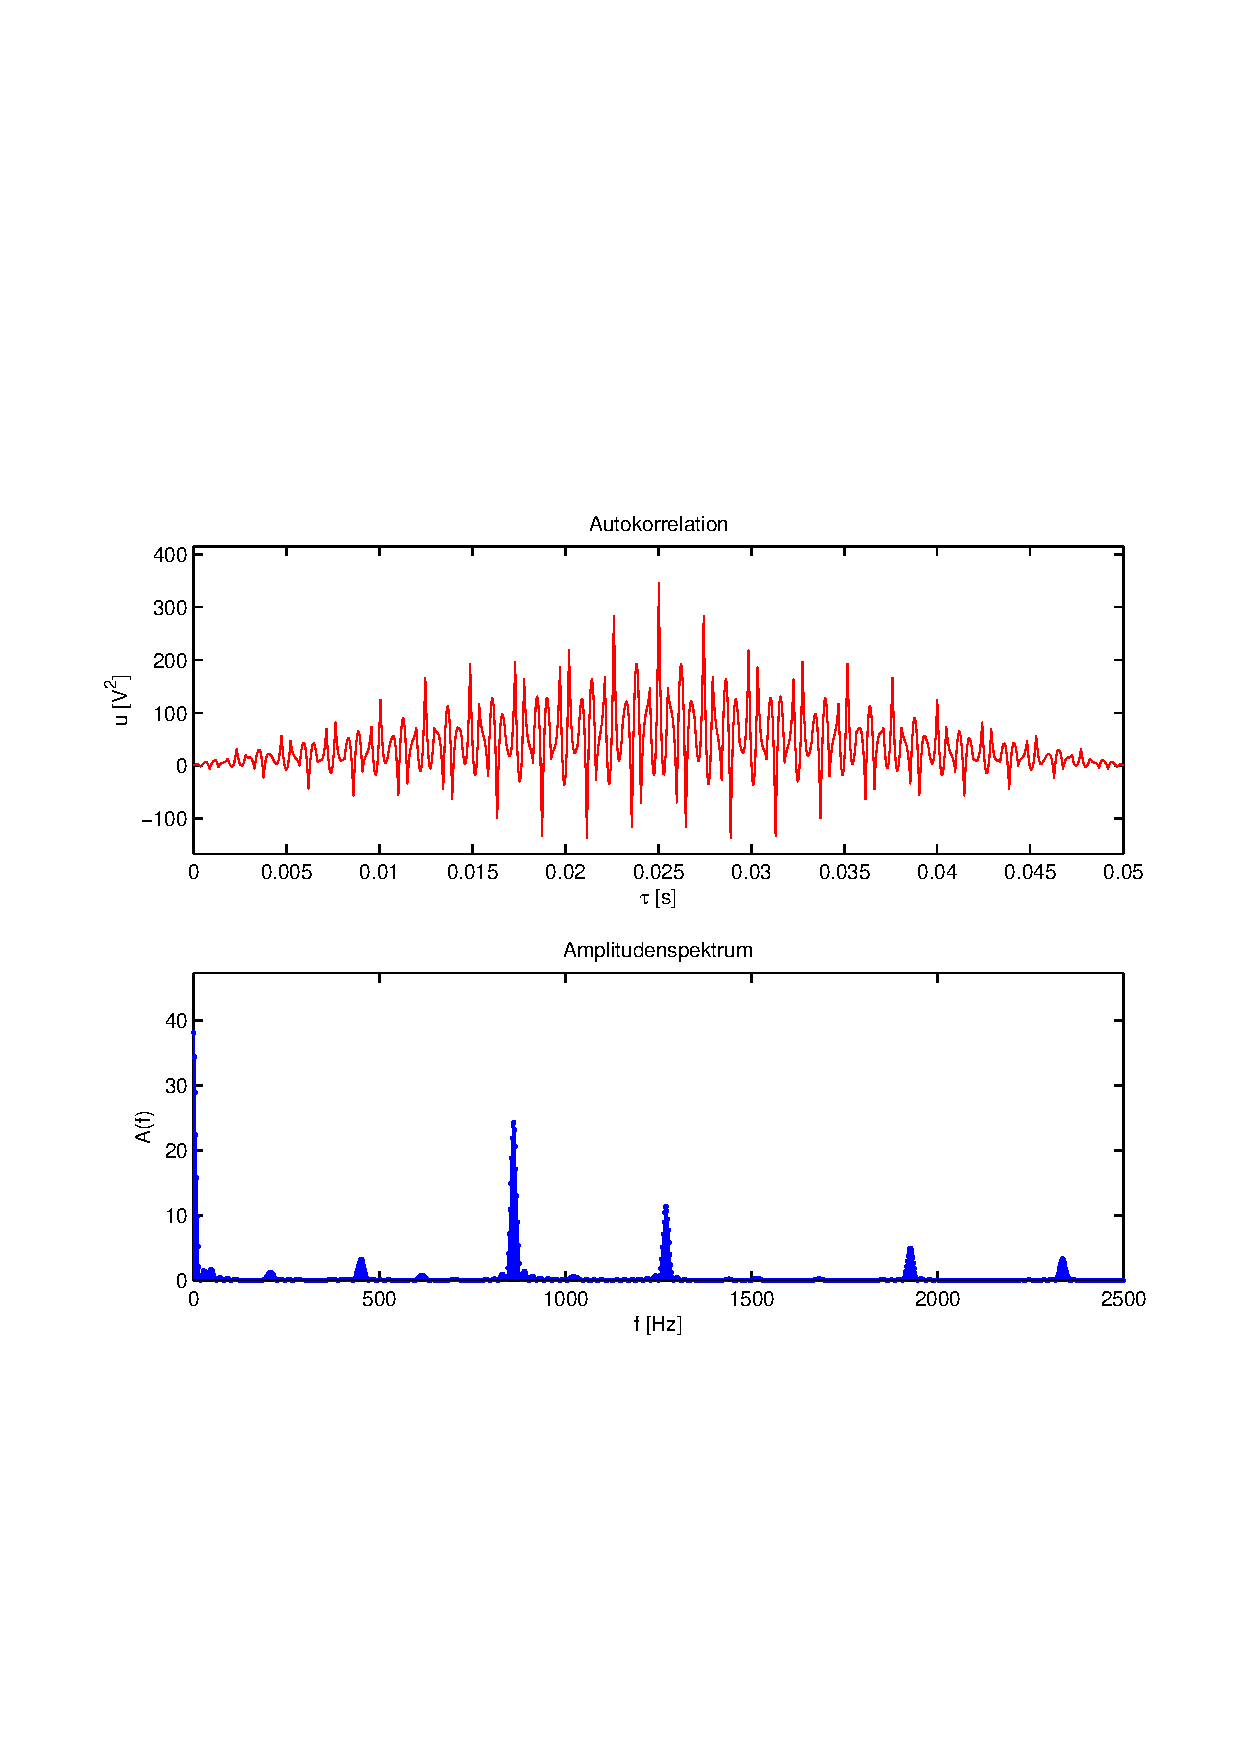
\includegraphics[scale=0.5, trim = 16mm 70mm 16mm 85mm, clip]
                                        {Bilder/8kHz_dreieck_LSD}
                        \caption{8 kHz Dreieck Quantisierungsfehler LDS}
                        \label{fig:8kHz_drei_LDS}
                    \end{figure}
                \end{minipage}
                
                \begin{minipage}{0.6\textwidth}
                    \begin{figure}[H]
                        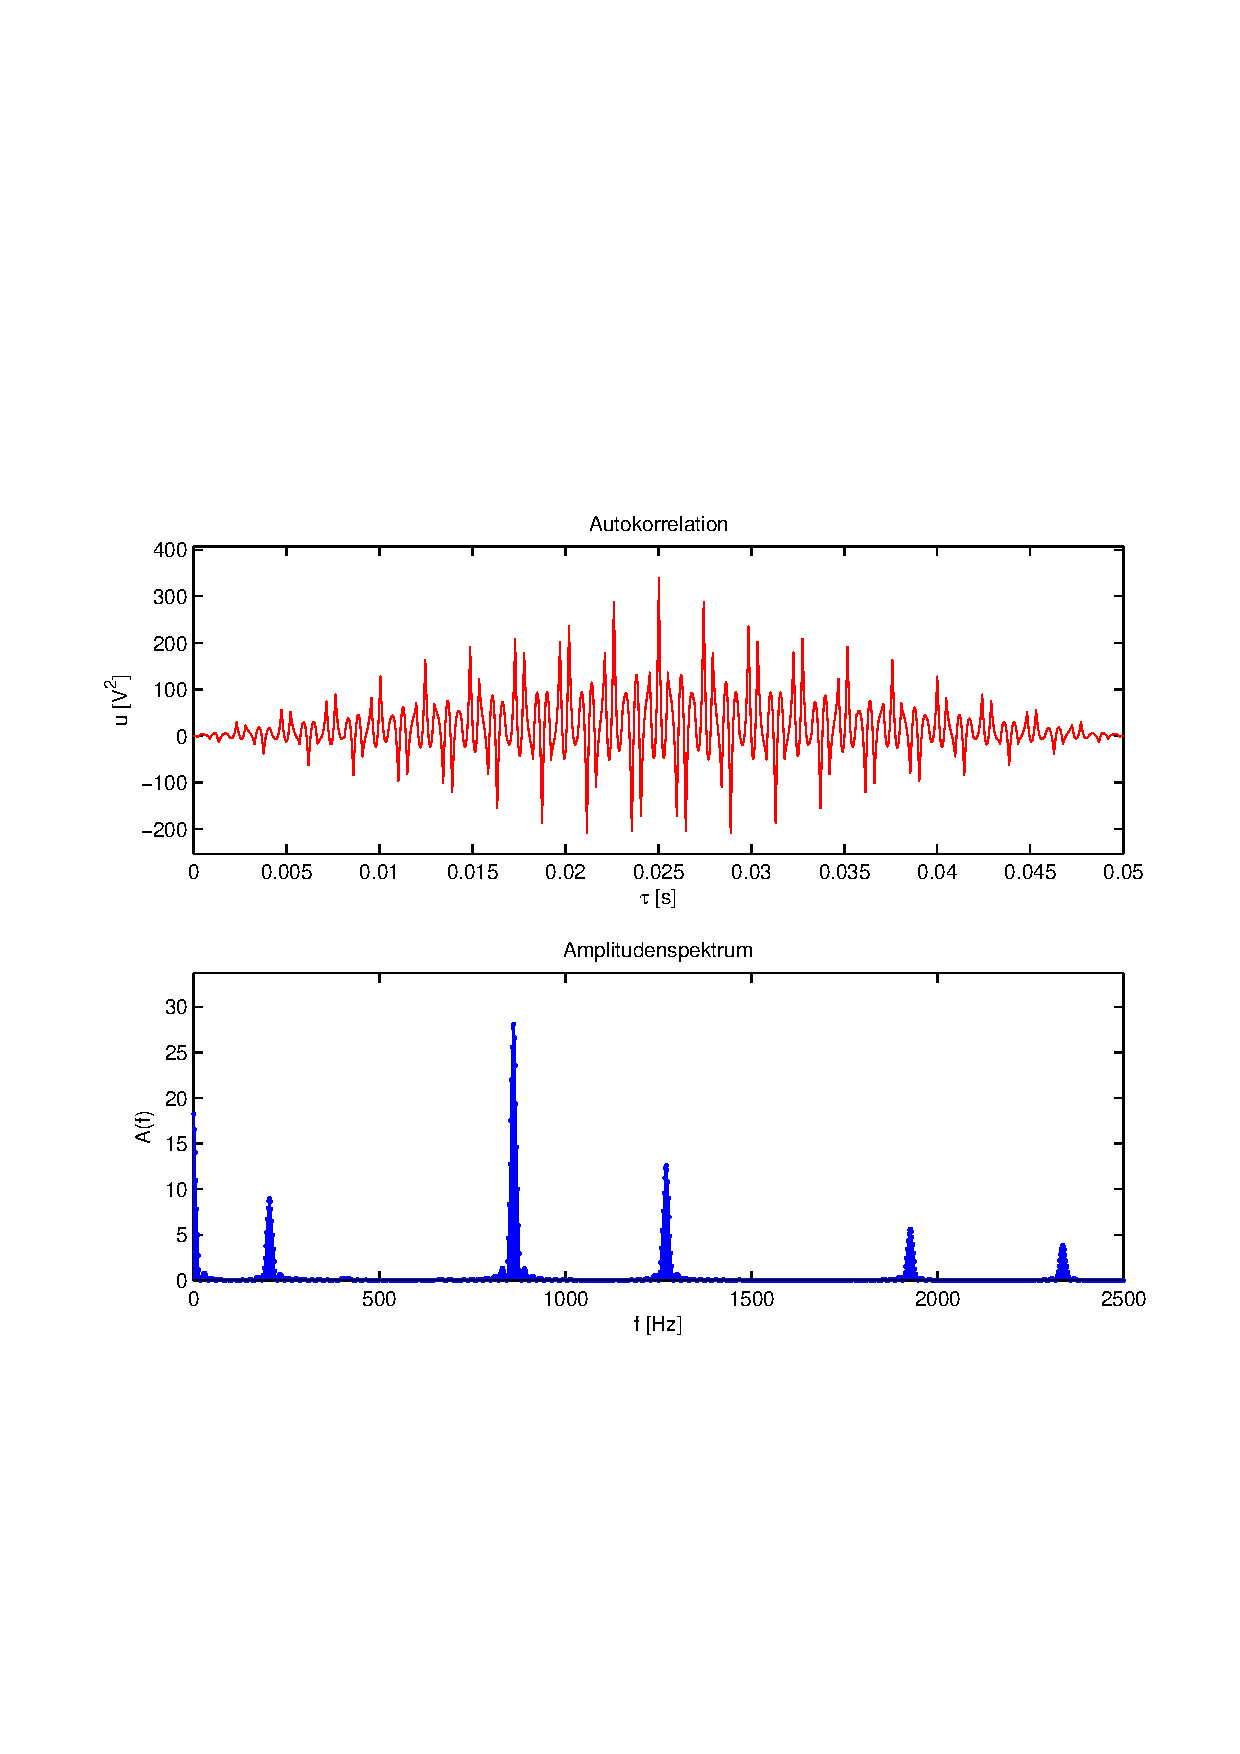
\includegraphics[scale=0.5, trim = 16mm 70mm 16mm 85mm, clip]
                                        {Bilder/8kHz_sin_LSD}
                        \caption{8 kHz Sinus Quantisierungsfehler LDS}
                        \label{fig:8kHz_sin_LDS}
                    \end{figure}
                \end{minipage}
            
            \end{tabular}
        \end{center}
        \vspace{2em}
        
        An den Spektren kann man erkennen, dass sich die Amplituden für die Abtastung mit 8 kHz deutlich höher sind, da
        der Quantisierungsfehler für eine kleinere Abtastfrequenz größer ist.
        
    \end{quote}
    
\end{quote}


\end{document}